The search for hints of supersymmetric particles is among the important goals of the LHC physics program. As discussed in Sec.~\ref{subsec:susy_collider}, searches performed at $\sqrt{s} = 7$\tev have constrained the allowed parameter space for light-flavour squarks and gluinos already up to around 800\gev and 1\tev for light LSP masses, respectively. However, the increased centre of mass energy from 7\tev to 8\tev and the recorded dataset which is around four times larger than at 7\tev provide the opportunity to extend the reach of such searches into entirely unexplored parameter regions. In Fig.~\ref{fig:susy_theory_xs} the theory cross section for the production of supersymmetric particles is shown as function of the SUSY particle mass. The y-axis on the right indicates how many events are expected in 20\fbinv of \pp collision data at the LHC at $\sqrt{s}=8$\tev. \\

\begin{figure}[!h]
  \centering
  \begin{tabular}{c}
                \includegraphics[width=0.65\textwidth]{figures/xsections_strong.pdf} 
  \end{tabular}
  \caption{Theory cross sections for selected SUSY processes as function of the SUSY sparticle mass. The y-axis on the right indicates the expected number of events in 20\fbinv of \pp collision data at the LHC at $\sqrt{s}=8$\tev~\cite{Kramer:2012bx}.}
  \label{fig:susy_theory_xs}
\end{figure}
It is visible that especially light-squarks and gluinos are expected at a sizable rate even for high masses above 1\tev. For instance, around 100 pairs of gluinos are expected at a mass of 1200\gev. \\
The analysis presented in this Chapter is aiming at a search for supersymmetric cascade decays arising from strongly produced light-flavour squarks or gluinos. Thus, events are selected based on the scalar sum of the jet transverse momenta (\HT), the missing transverse momentum calculated from the jet momenta (\MHT) and the number of jets (\NJets). However, the generic structure makes the analysis in principle sensitive to any new physics model that manifests in final states containing several hard jets accompanied by missing transverse energy. \\
After the description of the event selection (Sec.~\ref{sec:RA2_sel}), it is discussed how contributions from standard model processes to the selected final state are estimated. Special emphasis is put on the estimation of the QCD multijet background (Sec.~\ref{subsec:RA2_QCD}). Finally, results are presented and interpreted in various simplified supersymmetric models (Sec.~\ref{sec:RA2_results}). Parts of this Chapter are taken from~\cite{bib:AN-12-350}, having been written by the author. This analysis follows previous inclusive searches~\cite{springerlink:10.1007/JHEP08(2011)155, Chatrchyan:2012lia} and is published in~\cite{Chatrchyan:2014lfa}.    
\section{Event Selection}
\label{sec:RA2_sel}

\subsection{Data Samples and Trigger}
\label{subsec:RA2_samples_trigger}
The analysis is based on \pp collision data recorded with the CMS detector at a centre of mass energy of $\sqrt{s} = 8$\tev. This corresponds to an integrated luminosity of 19.5\fbinv for all sub-detectors fully functional. \\
The data have been collected by triggering on \HT, the scalar sum of the jet transverse momenta, and \met, the missing transverse energy. An overview of the considered runs and the integrated luminosity is shown together with the respective HLT trigger paths in Tab.~\ref{tab:RA2_trigger}. \HT and \met are calculated from particle-flow objects at trigger level with nominal thresholds of 350\gev and 100\gev, respectively. Jets considered in this calculation are reconstructed with the anti-$k_T$ algorithm and distance parameter $R = 0.5$. The labelling \textit{PFNoPU} indicates that for that particular runs also charged-hadron subtraction was applied to jets at trigger level. 
\begin{table}[!b]
\centering
\caption{Utilized signal trigger paths in individual run ranges listed together with the integrated luminosity.}
\label{tab:RA2_trigger}
 \makebox[\linewidth]{
\begin{tabular}{lccc}
\multicolumn{4}{c}{} \\
\toprule
 Trigger path & Run range & Luminosity [\fbinv] \\
\midrule
 HLT\_PFHT350\_PFMET100 & 190456 -- 196531 & 0.9 \\
 & & & \\
 HLT\_PFHT350\_PFMET100 & 190782 -- 190949 & 4.4 \\
 & & & \\
 HLT\_PFNoPUHT350\_PFMET100 & 198022 -- 198523 & 6.9 \\
 & & & \\
 HLT\_PFNoPUHT350\_PFMET100 & 198524 -- 208686 & 7.3 \\
\bottomrule
\end{tabular}}
\end{table}  
\\
In order to determine the offline values for \HT and \MHT (calculated according to the definition following in Sec.~\ref{subsec:RA2_baseline}) for which the triggers reach the plateau efficiency, the trigger efficiencies are measured with respect to a single electron trigger (HLT\_Ele27\_WP80). In principal, an orthogonal trigger is needed in order to get an unbiased estimate of the trigger efficiency. However, due to the PF-algorithm all subdetectors are used simultaneously to reconstruct the particles in an event. Hence, no independent trigger paths providing enough statistical precision are available. Consequently, only the reach of a plateau efficiency for a certain trigger path can be determined while the absolute efficiency is not accessible. The determination of the trigger plateau efficiency is performed for different jet multiplicity intervals (\NJets~$ = 3-5$, \NJets~$ = 6-7$ and \NJets~$ \ge 8$). The obtained trigger turn-on curves for the two different HLT paths are shown as function of offline \HT and \MHT for jet multiplicity \NJets~$ = 3-5$ in Fig.~\ref{fig:trig_eff_3njets5}. For both trigger paths, the efficiency plateau is reached around offline values of \HT$ = 500$\gev and \MHT$ = 200$\gev. The integrated trigger efficiencies for these particular values in different jet multiplicity intervals are summarized with statistical uncertainties in Tab.~\ref{tab:trig_eff}. In general, they are close to 100\% with small uncertainties below 1\%. However, for the highest jet multiplicity selection of \NJets~$ \ge 8$ only few events where selected such that statistical uncertainties are few 10\% large. Though, no hints for a systematic inefficiency have been observed and the signal triggers are considered as fully efficient with an uncertainty of $2\%$ for offline values of \HT$ > 500$\gev and \MHT$ > 200$\gev independent of the jet multiplicity. \\

\begin{figure}[!t]
  \centering
  \begin{tabular}{cc}
                \includegraphics[width=0.49\textwidth]{figures/turn_on_HT_TagEle27WP80_ProbePFHT350PFMET100_MHT200_chs_NJets3_5.png} &
                \includegraphics[width=0.49\textwidth]{figures/turn_on_MHT_TagEle27WP80_ProbePFHT350PFMET100_HT500_chs_NJets3_5.png} \\
                \includegraphics[width=0.49\textwidth]{figures/turn_on_HT_TagEle27WP80_ProbePFNoPUHT350PFMET100_MHT200_chs_NJets3_5.png} &
                \includegraphics[width=0.49\textwidth]{figures/turn_on_MHT_TagEle27WP80_ProbePFNoPUHT350PFMET100_HT500_chs_NJets3_5.png} \\
  \end{tabular}
\caption{Measured trigger efficiency for paths HLT\_PFHT350\_PFMET100 (\textit{top}) and HLT\_PFNoPUHT350\_PFMET100 (\textit{bottom}) as a function of \HT (\textit{left}) and \MHT (\textit{right}) shown for $3 \leq$ \NJets $\leq 5$.} 
  \label{fig:trig_eff_3njets5}
\end{figure}

\begin{table}[!t]
  \caption{Summary of total trigger efficiencies of the signal triggers for selections of offline \HT$ > 500$\gev and \MHT$ > 200$\gev in different jet multiplicity intervals.} 
  \label{tab:trig_eff}
  \begin{center}
    \begin{tabular}{lcc}
      \toprule
      \NJets & HLT\_PFHT350\_PFMET100 &  HLT\_PFNoPUHT350\_PFMET100\\
      \midrule
      3 - 5   & $99.4 _{-0.3} ^{+0.2}$   & $99.8 _{-0.1} ^{+0.1}$\\
      6 - 7   & $99.1 _{-2.0} ^{+0.7}$   & $100.0 _{-0.6} ^{+0.0}$\\
      $\ge$ 8 & $100.0 _{-36.9} ^{+0.0}$ & $100.0 _{-10.9} ^{+0.0}$\\
      \bottomrule
    \end{tabular}
  \end{center}
\end{table}

In order to validate the basic event selection discussed in Sec.~\ref{subsec:RA2_cleaning} and~\ref{subsec:RA2_baseline} and the background estimation methods described in Sec.~\ref{subsec:RA2_QCD} and~\ref{sec:RA2_Non-QCD}, several MC simulation samples are used. The standard model processes for \ttbar, \WJets, \ZJets, $\gamma + \mathrm{{jets}}$ and QCD multijet events are generated with the MadGraph5~\cite{Alwall:2007st} generator at leading order and are interfaced with the parton-shower model in Pythia 6.4.24~\cite{Sjostrand:2006za}. They are scaled to cross-section predictions at next-to-leading order or even next-to-next-to-leading order when available~\cite{Kidonakis:2010dk, Melnikov:2006kv}. The events are processed with the full detector simulation. Furthermore, SUSY signal samples are obtained from simulation. They are generated with MadGraph5~\cite{Alwall:2007st} (with up to two additional partons), the CTEQ6L parton distribution functions~\cite{Pumplin:2002vw} and processed with the fast detector simulation. Cross sections are determined at NLO with a resummation of soft gluon emission at the accuracy of next-to-leading-log~\cite{Beenakker:1996ch, PhysRevLett.102.111802, PhysRevD.80.095004, Beenakker:2009ha, Beenakker:2011fu, Kramer:2012bx}. The cross section calculation as well as the generation of signal events for a certain type of sparticle is performed by effectively removing contributions from other sparticles by assuming their mass to be very large.

\subsection{Event Cleaning}
\label{subsec:RA2_cleaning}
The analysis presented in this Chapter heavily realies on a precise measurement of the momentum imbalance in the event. In order to remove events with large values of fake missing momentum arising from detector noise a dedicated sequence of cleaning filters is applied. 
\begin{description}
 \item{\textbf{Primary Vertex and Beam Halo:}} Only events with at least one high-quality primary vertex are considered in the analysis. A primary vertex is classified as good, if it has more than four associated tracks and is located within 24\,cm in $z$ and 2\,cm in $xy$ direction from the nominal interaction point (\textit{good-vertex filter}). In order to reject events in which protons from the beam interact with residual gas molecules in the beam pipe, the CSC subdetector is used to identify muons moving parallel to the beam (\textit{beam-halo filter}).
 \item{\textbf{Anomalous Calorimeter Signals:}} Some events are affected by particles hitting the readout electronics or other technical instrumentation and cause anomalous signals in the ECAL or HCAL. For instance, noise in the readout system can fake artifical energy deposits at random times. Such events are identified based on timing and pulse-shape information (\textit{HBHE noise filter}). Furthermore, two $5 \times 5 $ supercrystal regions in the EE have been observed to give anomalously high energies. They are removed by imposing selections on the deposited energy in the identified supercrystals (\textit{EE bad supercrystal filter}). In order to account for transparency losses in the ECAL crystals, the system is calibrated with a dedicated laser. However, in the data some crystals are observed which receive unphysically large corrections. Events affected by this unusually large ECAL laser correction factors are rejected (\textit{ECAL laser correction filter}). The HCAL is also monitored by a dedicated laser system. Sometimes the laser fires into the collision bunch-crossing resulting in unwanted signals. These events are removed according to an event list indicating the affected events (\textit{HCAL laser filter}). The jet reconstruction utilizes information from the HO. This is used as identifier of significant leakage beyong the HCAl barrel. However, events with anomalous energy deposits in the HO have to be rejected. Thus, events in which the fraction of the momentum deposited in the HO is $> 40\%$ are removed (\textit{HO filter}).
 \item{\textbf{Dead ECAL Cells:}} Some single crystals in the ECAL are affected by malfunctioning. These single dead ECAL cells make up around $1\%$ in total and can be responsible for energy losses resulting in large values of fake-\MHT. Such events can be identified by using the trigger primitive information to determine how much energy was lost (\textit{TP filter}) or by using the surrounding energy of the masked cells (\textit{BE filter}).
 \item{\textbf{Tracking Failure:}} In some events the track reconstruction is observed to fail manifesting in large calorimeter energy deposits with lack of associated tracks. This can be caused e.g. by too many seed clusters or by collisions not taking place in the actual center of the detector. Thus, the scalar sum of track momenta associated to the good vertices divided by \HT in the event has to be larger than 10\% (\textit{tracking failure filter}) and if at least ten tracks are present in the event, good-quality tracks have to be more than 25\% (\textit{beam-scraping filter}). In addition, events with misreconstructed muon momenta in the PF algorithm (\textit{inconsistent muon filter}) or events where soft muons wrongly absorb energy from energetic HCAL towers they traverse (\textit{greedy muon filter}) are rejected. Furthermore, events with coherent noise in the strip tracker can occur. These cause several clusters distributed across the whole detector and lead to the identification of fake tracks. Such events where the track reconstruction aborted can be identified by comparing the number of pixel clusters to the number of strip clusters (\textit{many strip clusters filter}, \textit{too many strip clusters filter}, \textit{log error too many strip clusters filter}). Another failure of track reconstruction occurs sometimes when track seeds from the TOB and TEC are used. Consequently, events are rejected, if a jet with number of charged hadrons above 200 is reconstructed within $0.9 < |\eta| < 1.9$ (\textit{TOB/TEC tracking filter}).
 \item{\textbf{Noise Induced Jets:}} In order to reject events with fake jets from detector noise, events are discarded if the energy of a jet with \pt$ > 30$\gev is composed of more than 95\% from PF photon candidates or more than 90\% from PF neutral hadron energy (\textit{PBNR filter}).
\end{description}

\subsection{Baseline Selection}
\label{subsec:RA2_baseline}
The physics objects used in the analysis are reconstructed with the PF algorithm. Jets are clustered from the particle-flow objects with the anti$-k_T$ algorithm using $R = 0.5$. Furthermore, they are calibrated as discussed in Sec.~\ref{subsec:jets_calib} including residual correction factors for data. \\
The following \textit{baseline selection} criteria are used to pre-define the event sample used for the analysis.
\begin{itemize}
 \item{The number of jets (\NJets) is required to be $\ge 3$. \NJets is defined as the number of jets with $\pt > 50$\gev and $|\eta| < 2.5$. This requirement is imposed in order to select multijet events.}
 \item{The scalar sum of jet momenta (\HT) is required to be $\ge 500$\gev with 
\begin{equation*}
\HT = \sum_{\mathrm{jets}} \pt 
\end{equation*}
for all jets that have $\pt > 50$\gev and $|\eta| < 2.5$. This condition selects events with a large visible energy in the event indicating a high energy scale of the hard interaction.}   
 \item{The absolute value of the negative vectorial sum of the jet momenta (\MHT) is required to be $\ge 200$\gev with
\begin{equation*}
\MHT = |\MHTvec|= |- \sum_{\mathrm{jets}} \ptvec|
\end{equation*}
for all jets with $\pt > 30$\gev and $|\eta| < 5.0$. This selection reduces contributions from standard model processes where missing transverse momentum is expected to be small. Especially, QCD multijet background is suppressed. } 
 \item{In order to suppress events where missing transverse energy is mainly arising from jet mismeasurements, as for QCD multijet events, it is required that \MHT is not aligned with the leading three jets. Thus, events with
\begin{equation*}
\Delta \phi(\mathrm{jet}_n, \MHT) > 0.5 \;\; \mathrm{for} \;\; n = 1,2 \;\; \mathrm{and} \;\; \Delta \phi(\mathrm{jet}_3, \MHT) > 0.3
\end{equation*} 
are selected. The value of 0.5 is chosen according to the jet size parameter. However, this is reduced in case of the third jet in order to retain signal efficiency. }
 \item{Background contributions arising from \ttbar and \WJets events are reduced by rejecting events containing isolated electrons or muons with $\pt > 10$\gev. These are required to have a good quality track that can be associated with the primary interaction vertex~\cite{CMS-PAS-EGM-10-004, CMS-PAS-MUO-10-002}. The isolation is given as the scalar sum of transverse momenta of PF particles (except for the lepton itself) within a cone of width $\Delta R = 0.3$ for the electron and $\Delta R = 0.4$ for the muon, respectively. This is required to be less than 15\% of the transverse momentum of the electron and less than 20\% of the transverse momentum of the muon.}
\end{itemize}
The selection described above defines a loose validation region and provides a basis for tighter criteria. In data, 11753 events are selected after the application of the baseline selection including the event cleaning filters. A comparison of selected events in data and simulation after the basline selection is shown in Fig.~\ref{fig:ra2_baseline_mc}. Although a reasonable data and MC agreement is observed especially in the bulk of the distributions, the background estimation from simulation is not further used in the analysis, but is meant to give an impression of the relative background contributions. Since the analysis is performed in extreme tails of the \HT, \MHT and \NJets phase space with only few events and large theoretical uncertainties in the simulation, SM background contributions are estimated solely with data-based methods.

\begin{figure}[!t]
  \centering
  % \makebox[\linewidth]{
  \begin{minipage}[c]{1.\textwidth}
    \begin{center}
      \includegraphics[width=0.49\textwidth]{figures/RA2_baseline_MC_HT.pdf}  
      \includegraphics[width=0.49\textwidth]{figures/RA2_baseline_MC_MHT.pdf} \\
      \includegraphics[width=0.49\textwidth]{figures/RA2_baseline_MC_NJets.pdf}
    \end{center}
  \end{minipage}

  \caption{Comparison of selected \HT (\textit{top left}), \MHT (\textit{top right}) and \NJets (\textit{bottom}) distributions in data (\textit{black dots}) and simulated events (\textit{shaded curve}) found from applying the event cleaning and baseline selection criteria described in Sec.~\ref{subsec:RA2_cleaning} and~\ref{subsec:RA2_baseline}. Only statistical uncertainties are shown. Taken from~\cite{Chatrchyan:2014lfa}.}
  \label{fig:ra2_baseline_mc}
\end{figure}

\subsection{Exclusive Search Regions}
\label{subsec:RA2_search_regions}
The analysis presented in this Chapter is an extension of previous inclusive searches~\cite{springerlink:10.1007/JHEP08(2011)155, Chatrchyan:2012lia}. These have been based on the requirement of at least three jets in the final state. In this analysis, the data is further subdivided into three exclusive jet multiplicity categories: $\NJets = 3 - 5, 6 - 7, \ge 8$. This enhances the sensitivity of the search towards multijet final states. These are typically the manifestations of long cascade decays from squarks and gluinos. Furthermore, it enlarges the sensitivity of the analysis to models in which gluinos often decay into top quarks. By requiring a large number of jets this analysis utilizes a complementary approach to other analyses which often use the presence of bottom-quark jets in the final state to discriminate against background~\cite{Chatrchyan:2013lya, Chatrchyan:2013wxa, CMS-PAS-SUS-13-019, CMS-PAS-SUS-14-011}. This procedure allows to keep the signal efficiency for all-hadronic final states as high as possible. In order to gain sensitivity to a variety of models, the jet categories are further classified according to \HT and \MHT. With this approach various exclusive search regions are defined. An overview of the exact definition of all 36 exclusive regions in \NJets, \HT and \MHT is given in Tab.~\ref{tab:excl_search_bins}.

\begin{table}[!h]
%\fontsize{10 pt}{1.2 em}
%\selectfont
\centering
\caption{Exclusive search regions used in the analysis binned in \HT, \MHT and \NJets.}
\begin{tabular}{lccc}
\multicolumn{4}{c}{} \\
  \toprule
   \NJets & [3-5] & [6-7] & [$\geq$8]  \\
  \midrule
             & \MHT [\gev]  & \MHT[\gev]  & \MHT[\gev]       \\
  \midrule
   500 $<$ \HT [\gev] $<$ 800   & 200-300 & 200-300 & $>$ 200 \\
                     & 300-450 & 300-450 &        \\
                     & 450-600 & $>$ 450  &        \\
                     & $>$ 600 &         &        \\
  \midrule
   800 $<$ \HT [\gev] $<$ 1000  & 200-300 & 200-300 & $>$ 200 \\
                     & 300-450 & 300-450 &        \\
                     & 450-600 & $>$ 450  &        \\
                     & $>$ 600 &         &        \\
  \midrule
   1000 $<$ \HT [\gev] $<$ 1250 & 200-300 & 200-300 & $>$ 200 \\
                     & 300-450 & 300-450 &        \\
                     & 450-600 & $>$ 450  &        \\
                     & $>$ 600 &         &        \\
  \midrule
   1250 $<$ \HT [\gev] $<$ 1500 & 200-300 & 200-300 & $>$ 200 \\
                     & 300-450 & 300-450 &        \\
                     & $>$ 450 & $>$ 450 &        \\
  \midrule
  \HT [\gev] $>$ 1500         & 200-300 & 200-300 & $>$ 200 \\
                     & $>$ 300  & $>$ 300  &        \\
  \bottomrule
\end{tabular}
\label{tab:excl_search_bins}
\end{table}    

\section{Estimation of Non-QCD Backgrounds}
\label{sec:RA2_Non-QCD}
As discussed in Sec.~\ref{subsec:susy_collider}, events from the SM processes \ZInvJets, \WJets or semi-leptonic \ttbar (where either the lepton is lost or a hadronically decaying $\tau$ lepton) and mismeasured QCD multijet events constitute important background contributions to all-hadronic final states. Dedicated data-based methods are employed to estimate their size in the selected data. In this Section those methods are described starting with a short review of the estimation of non-QCD backgrounds (Sec.~\ref{subsec:RA2_Zinv}, Sec.~\ref{subsec:RA2_tauhad} and Sec.~\ref{subsec:RA2_lostlepton}) followed by a detailled discussion of the QCD background estimation (Sec.~\ref{subsec:RA2_QCD}). 

\subsection{Invisible Z Background}
\label{subsec:RA2_Zinv}
\begin{figure}[!t]
  \centering
\makebox[\linewidth]{
  \begin{tabular}{cc}
                \includegraphics[width=0.49\textwidth]{figures/RA2_Zinv1.pdf} & 
                \includegraphics[width=0.49\textwidth]{figures/RA2_Zinv2.pdf} \\
                \includegraphics[width=0.49\textwidth]{figures/RA2_Zinv3.pdf} &
                \includegraphics[width=0.49\textwidth]{figures/RA2_Zinv4.pdf}
  \end{tabular}}
  \caption{The simulated ratio $R_{Z/\gamma}$ as a function of (a) \MHT, (b) \HT, (c) \NJets, where the values for three \MHT selections are shown with linear fits, and (d) the double ratio of $R_{Z(\mu+\mu-)/\gamma}$, using events from data to those from simulation; the linear fit and its uncertainty band are overlaid. Taken from~\cite{Chatrchyan:2014lfa}.}
  \label{fig:ra2_zinv}
\end{figure}
The irreducible background contributions arising from \ZInvJets events are estimated using \photonJets events. This is a well suited method as for high transverse momenta of the vector boson the event kinematics are basically the same and the cross sections differ only according to the different couplings~\cite{Ask:2011xf, Bern:2012vx}. \\
The \photonJets sample is collected by triggering on a $\photon$ candidate and large values of \HT. Photon candidates are selected if they satisfy \pt$ > 100$\gev and $|\eta| < 1.44$ or $1.566 < |\eta| < 2.5$. Furthermore, they have to have a shower profile consistent with that of a prompt photon produced directly in the hard interaction. In order to distinguish photons from misidentified electrons they must not have an associated track in the pixel detector. In addition, photon candidates are required to be isolated meaning that in a cone of $\Delta R = 0.3$ the summed transverse momenta of PF candidates around the momentum direction of the photon candidate are not allowed to exceed a certain value. The number of selected \photonJets events is corrected for photon acceptance, reconstruction and isolation efficiency. Furthermore, the purity of the \photonJets sample which is the fraction of selected photon candidates emerging from direct production has to be taken into account. The number of background photons caused \eg by misidentified jet fragments, is estimated by exploiting the difference between the shower profile of prompt and background photons. The average purity of the \photonJets sample is measured to be 93\%.\\
Subsequently, the number of \ZInvJets events in data $N_{\ZInvJets}^{\text{data}} (\HT, \MHT, \NJets)$ using the number of selected \photonJets events $N_{\photonJets}^{\text{data}} (\HT,\MHT,\NJets)$ is obtained according to
\begin{equation*}
N_{\ZInvJets}^{\text{data}} (\HT, \MHT, \NJets) = R^{\text{MC}}_{Z(\nu\bar{\nu})/\gamma} (\HT,\MHT,\NJets)
                                                        \times 
                                                       \frac{R_{Z(\mu\mu)/\gamma}^{\text{data}}}{R_{Z(\mu\mu)/\gamma}^{\text{MC}}}
                                                        \times 
                                                       N_{\photonJets}^{\text{data}} (\HT,\MHT,\NJets)
\label{eqn:photoncorr}
\end{equation*}
with the ratio relating the production cross section of \ZInvJets and \photonJets events $R^{\text{MC}}_{Z(\nu\bar{\nu})/\gamma} (\HT,\MHT,\NJets)$ determined in simulation and the double ratio $\frac{R_{Z(\mu\mu)/\gamma}^{\text{data}}}{R_{Z(\mu\mu)/\gamma}^{\text{MC}}}$ selected in data and MC to consider the theoretical uncertainty and correct $R_{Z/\gamma}$ for a given jet multiplicity. The missing momentum in the event is emulated by ignoring the momentum of the photon candidate in the calculation of \MHT. \\
The behaviour of $R_{Z/\gamma}$ is examined in simulated events as function of \MHT, \HT and \NJets. The obtained distributions are shown in Fig.~\ref{fig:ra2_zinv}\,(a) -- (c). While a strong dependence on \MHT for small values ($\lesssim 500$\gev) is observed, the variation as function of \HT amounts to only $(12 \pm 5)\%$ in the relevant range for this analysis of $\HT = 500 - 1500$\gev. The ratio as function of the jet multiplicity is determined for different \MHT ranges of $\MHT = 200 - 300$\gev, $\MHT = 300 - 450$\gev and $\MHT > 450$\gev. The behaviour in each of these \MHT ranges is described by a linear function also displayed in Fig.~\ref{eqn:photoncorr}\,(c). It is found that the ratio decreases slightly with increasing jet multiplicity which is consistent with findings from theory~\cite{Bern:2012vx, Bern:2011pa}. \\
In order to take the theoretical uncertainty on $R_{Z/\gamma}$ into account this phenomenological ratio is also determined for $Z_{\mu^+\mu^-}$ events in data and simulation, respectively. The double ratio of $R_{Z(\mu\mu)/\gamma}^{\text{data}}$ to $R_{Z(\mu\mu)/\gamma}^{\text{MC}}$ is derived as function of the jet multiplicity and shown in Fig.~\ref{eqn:photoncorr}\,(d). It is fitted with a linear function and the deviation from unity is considered as correction for the $R_{Z/\gamma}$ ratio in each jet multiplicity selection. \\
The main sources of uncertainty for the prediction of \ZInvJets events arise from the fit uncertainty to the double ratio which is at the order of 20\%, 25\% and 45\% for the different jet multiplicity intervals, the differences between data and simulation regarding the photon identification and isolation as well as the subtraction of background photons from QCD multijet events.

\subsection{Hadronic $\tau$ Background}
\label{subsec:RA2_tauhad}
\begin{figure}[!t]
  \centering

  \begin{minipage}[c]{1.\textwidth}
    \begin{center}
      \includegraphics[width=0.49\textwidth]{figures/RA2_TauHad1.pdf}% \hspace {1.5 pt} 
      \includegraphics[width=0.49\textwidth]{figures/RA2_TauHad2.pdf}\\ 
      \includegraphics[width=0.49\textwidth]{figures/RA2_TauHad3.pdf}
    \end{center}
  \end{minipage}

  \caption{Predicted (a) \HT, (b) \MHT, and (c) \NJets distributions found from applying the hadronic-tau background evaluation method to simulated \ttbar and \WJets events (solid points) in comparison to the genuine \ttbar and \WJets background from simulation (shaded curve). Only statistical uncertainties are shown. Taken from~\cite{Chatrchyan:2014lfa}.}
  \label{fig:ra2_tauhad}
\end{figure}
Background contributions arising from \WJets and \ttbar events with a hadronically decaying $\tau$ lepton are estimated using a $\mu + \mathrm{jets}$ control sample. Since $\mu + \mathrm{jets}$ and $\tau_h + \mathrm{jets}$ events arise from the same physics process, they feature the same kinematics except for the different response of the detector to a $\mu$ and a $\tau_h$.  \\
The $\mu + \mathrm{jets}$ sample is selected by triggering on a single muon or a muon accompanied by at least two jets. Furthermore, instead of applying a lepton veto, exactly one $\mu$ with \pt$ > 20$\gev and $|\eta| < 2.1$ is required. In order to prevent the control sample from signal contamination a selection on the transverse mass $m_T = \sqrt{2\pt^{\mu}\met[1-\mathrm{cos(\Delta \phi)}]}$ of $m_T \le 100$\gev is imposed with the azimuthal angle $\Delta \phi$ between the direction of the muon four-momentum and the \met vector. \\
The difference between the $\mu$ and the $\tau_h$ is taken into account by replacing the muon by a simulated $\tau_h$ jet. This is done by randomly sampling the transverse momentum of the $\tau_h$ jet from the response $\pt^\mathrm{jet}/\pt^{\tau}$ obtained from simulation a reconstructed jet with $\pt^\mathrm{jet}$ to a generated hadronically decaying $\tau$ lepton with $\pt^{\tau}$ in the $(\eta, \phi)$-space. The generated $\tau$ lepton has to fulfill $\pt > 20$\gev and $|\eta| < 2.1$ and the distance for the matching is chosen to be $\Delta R < 0.2$ for tau-\pt$ < 50$\gev and $\Delta R < 0.1$ otherwise. The response is obtained from simulated \ttbar and \WJets events and subsequently mixed according to the cross sections of these processes in order to emulate what happens in data where both \ttbar and \WJets events occur. The random sampling of the response is repeated one hundred times for each event to sample the complete response function. If an event in the control sample is obtained from a prescaled trigger, the repetition of the sampling is increased according to the prescale factor. Technically, sampling means that the four-momentum of the muon is sclaed with the proper value from the $\tau_h$ response.  \\
In the following, \HT, \MHT and \NJets are recalculated for each event including the transverse momentum of the $\tau_h$ jet and all selection criteria as described in Sec.~\ref{subsec:RA2_baseline} are applied to the sample. The background contribution due to hadronic-$\tau$ events is obtained for all search regions by further correcting the event yields for the trigger efficiency, muon reconstruction and isolation efficiency, kinematic and detector acceptance as well as the ratio of branching fractions of $W \rightarrow \tau_h \nu$ to $W \rightarrow \mu \nu$ events. The statistical uncertainty of the background prediction is estimated with pseudo-experiments using a bootstrap method~\cite{GVK017474957}. \\
The validity of this background estimation procedure is tested by comparing the event yields obtained from applying the prediction method to simulated events from \ttbar and \WJets events to the respective genuine background. This comparison is shown as function of \HT, \MHT and \NJets in Fig.~\ref{fig:ra2_tauhad} after the baseline selection. Although the agreement is quite reasonable and hence the method is supposed to work reliable, uncertainties of 10\% are considered for $\NJets = 3 - 5$ and 20\% for jet multiplicities $\NJets = 6 - 7$ and $\NJets \ge 8$. These uncertainties mainly reflect the statistical precision of the validation test. \\
Further systematic uncertainties taken into account for the hadronic $\tau$ background prediction are covering differences in data and MC for the muon isolation and reconstruction efficiencies as well as uncertainties on the kinematic and geometric acceptance, the $\tau_h$ jet response and the acceptance of the transverse mass cut. 

%\begin{figure}[!t]
%  \centering
%\makebox[\linewidth]{
%  \begin{tabular}{ccc}
%                \includegraphics[width=0.4\textwidth]{figures/RA2_TauHad1.pdf} & 
%                \includegraphics[width=0.4\textwidth]{figures/RA2_TauHad2.pdf} &
%                \includegraphics[width=0.4\textwidth]{figures/RA2_TauHad3.pdf}
%  \end{tabular}}
%  \caption{Predicted (a) \HT, (b) \MHT, and (c) \NJets distributions found from applying the hadronic-tau background evaluation method to simulated \ttbar and \WJets events (solid points) in comparison to the genuine \ttbar and \WJets background from simulation (shaded curve). Only statistical uncertainties are shown. Taken from~\cite{Chatrchyan:2014lfa}.}
%  \label{fig:ra2_tauhad}
%\end{figure}

\subsection{Lost-Lepton Background}
\label{subsec:RA2_lostlepton}
\begin{figure}[!t]
  \centering

  \begin{minipage}[c]{1.\textwidth}
    \begin{center}
      \includegraphics[width=0.49\textwidth]{figures/RA2_LL1.pdf}% \hspace {1.5 pt} 
      \includegraphics[width=0.49\textwidth]{figures/RA2_LL2.pdf}\\ 
      \includegraphics[width=0.49\textwidth]{figures/RA2_LL3.pdf}
    \end{center}
  \end{minipage}

  \caption{Predicted (a) \HT, (b) \MHT, and (c) \NJets distributions found from applying the lost lepton background evaluation method to simulated \ttbar and \WJets events (solid points) in comparison to the genuine \ttbar and \WJets background from simulation (shaded curves). Only statistical uncertainties are shown. Taken from~\cite{Chatrchyan:2014lfa}.}
  \label{fig:ra2_ll}
\end{figure}
Similar to background events from hadronic tau decays, the background contribution due to a failed veto of a light lepton is estimated from a $\mu + \mathrm{jets}$ control sample. This is selected with the same trigger as used for the search. The sample is selected by requiring exactly one well-reconstructed and isolated muon with $\pt > 10$\gev. Furthermore, the same transverse mass requirement of $m_T < 100$\gev as for the hadronic tau background is applied. \\ 
The number of events in the zero-lepton search regions can be estimated from the single-muon sample by weighting the events according to the lepton reconstruction and isolation efficiencies as well as the detector and kinematic acceptance of the muons. The respective efficiencies and acceptances are obtained from simulated \ttbar and \WJets events and determined in intervals of \HT, \MHT and \NJets. \\
In order to determine the number of events due to unidentified leptons the events in the control sample are weighted according to
\begin{equation*}
\frac{1}{\epsilon_\mathrm{iso}^\mathrm{\mu}} \times \frac{1-\epsilon_\mathrm{reco}^{e, \mu}}{\epsilon_\mathrm{reco}^{\mu}}
\end{equation*}
and with
\begin{equation*}
\frac{\epsilon_\mathrm{reco}^{e, \mu}}{\epsilon_\mathrm{reco}^{\mu}} \times \frac{1-\epsilon_\mathrm{iso}^{e, \mu}}{\epsilon_\mathrm{iso}^{\mu}}
\end{equation*}
to account for non-isolated leptons. Both equations are based on the reconstruction $\epsilon_\mathrm{reco}^{e, \mu}$ and isolation $\epsilon_\mathrm{iso}^{e, \mu}$ efficiencies of the electron and muon, respectively. 
The method is validated in simulation by comparing the predicted event yields for lost-lepton events in \ttbar and \WJets from a signle-muon control sample after the baseline selection to the genuine background. This comparison is illustrated in Fig.~\ref{fig:ra2_ll} as function of \HT, \MHT and \NJets and shows a good overall agreement. An uncertainty of 15\% is assigned to jet multiplicities 3--5 and 40\% to the others in order to account for the statistical precision of this validation test.\\
Main other uncertainties of the lost-lepton background prediction arise from the lack of sufficient events in the control sample in each defined search region, differences in lepton reconstruction and isolation efficiency between data and simulation, impact on the acceptance when varying the used PDFs and the acceptance of the transverse mass cut.

%\begin{figure}[!t]
%  \centering
%\makebox[\linewidth]{
%  \begin{tabular}{ccc}
%                \includegraphics[width=0.4\textwidth]{figures/RA2_LL1.pdf} & 
%                \includegraphics[width=0.4\textwidth]{figures/RA2_LL2.pdf} &
%                \includegraphics[width=0.4\textwidth]{figures/RA2_LL3.pdf}
%  \end{tabular}}
%  \caption{Predicted (a) \HT, (b) \MHT, and (c) \NJets distributions found from applying the lost lepton background evaluation method to simulated \ttbar and \WJets events (solid points) in comparison to the genuine \ttbar and \WJets background from simulation (shaded curves). Only statistical uncertainties are shown. Taken from~\cite{Chatrchyan:2014lfa}.}
%  \label{fig:ra2_ll}
%\end{figure}

\section{QCD Background Estimation with the Rebalance-And-Smear Method}
\label{subsec:RA2_QCD}
Background contributions arising from events with no intrinsic missing energy, except for neutrinos in jets arising for instance from electroweak decays of heavy-flavour quarks, are estimated with the \textit{Rebalance-and-Smear} (R+S) method. The main contribution is caused by QCD multijet events which also caused the naming 'QCD background'. However, minor contributions originate also from fully-hadronic decaying \ttbar, \WJets and \ZJets events. The high values of missing transverse energy which cause these events to contribute to the analysed signal regions is consequently arising from severe jet mismeasurements. \\
Typically, QCD background is the most difficult background to model for all-hadronic SUSY searches, as a precise description of the underlying particle-level jet spectrum is needed and how this manifests in the detector. Especially the former suffers from large theoretical uncertainties in particular in the extreme kinematic phase space the analysis is performed in. To overcome this, the data-based R+S-method was developed and already successfully used in previous analyses~\cite{springerlink:10.1007/JHEP08(2011)155, Chatrchyan:2012lia}. In this thesis, particularly improvements of the R+S method are discussed that became inevitable to handle the main changes of this analysis at $\sqrt{s} = 8$\tev manifesting in the extension of the search regions in several jet mulitplicities and the increased amount of pileup compared to the 7\tev analyses. Consequently, the R+S method is adjusted such that it leads to precise results regarding also this new conditions. In general, the method is based on the assumption that if the momenta of particle-level jets in an event are known, the reconstructed jet momenta can be modeled by a per-jet resolution function.  \\
After the discussion of the general concept of the R+S method in Sec.~\ref{subsec:RPlusS_concept}, the adjustment of the procedure to the actual conditions for 8\tev data are introduced in Sec.~\ref{subsec:RPlusS_app}. Furthermore, systematic uncertainties are discussed in Sec.~\ref{subsec:RA2_syst_unc} and the results of the actual QCD background prediction are presented in Sec.~\ref{subsec:RA2_qcd_pred}. 

\subsection{General concept of the Rebalance-and-Smear method}
\label{subsec:RPlusS_concept} 
As stated above, QCD background contributions arise from jet mismeasurements in the detector. Thus, this background contribution can be estimated by retracing the measurement of multijet events. In order to do this, the prediction of the QCD background is performed in two subsequent steps. First, the events are rebalanced, as described below, such that the missing energy in the event is removed and almost ideal multijet events denoted \textit{seed events} are obtained. The resulting seed events reflect the event kinematics before the actual detector measurement is performed and are thus estimators of the true particle-level jet momenta. In a second step, all jets in the event are smeared with the full jet response function, \ie jet momenta are scaled with a factor randomly drawn according to the jet response distribution, to model the interaction of the multijet state with the detector. Smeared events contain the whole event kinematics of the studied background contribution, such that these can be used to derive contributions to various kinematic distributions, like \HT or \MHT. The general outline of the R+S method is illustrated in Fig.~\ref{fig:RPlusS_concept}.
\begin{figure}[!t]
  \centering
  \makebox[\linewidth]{
  \begin{tabular}{c}
                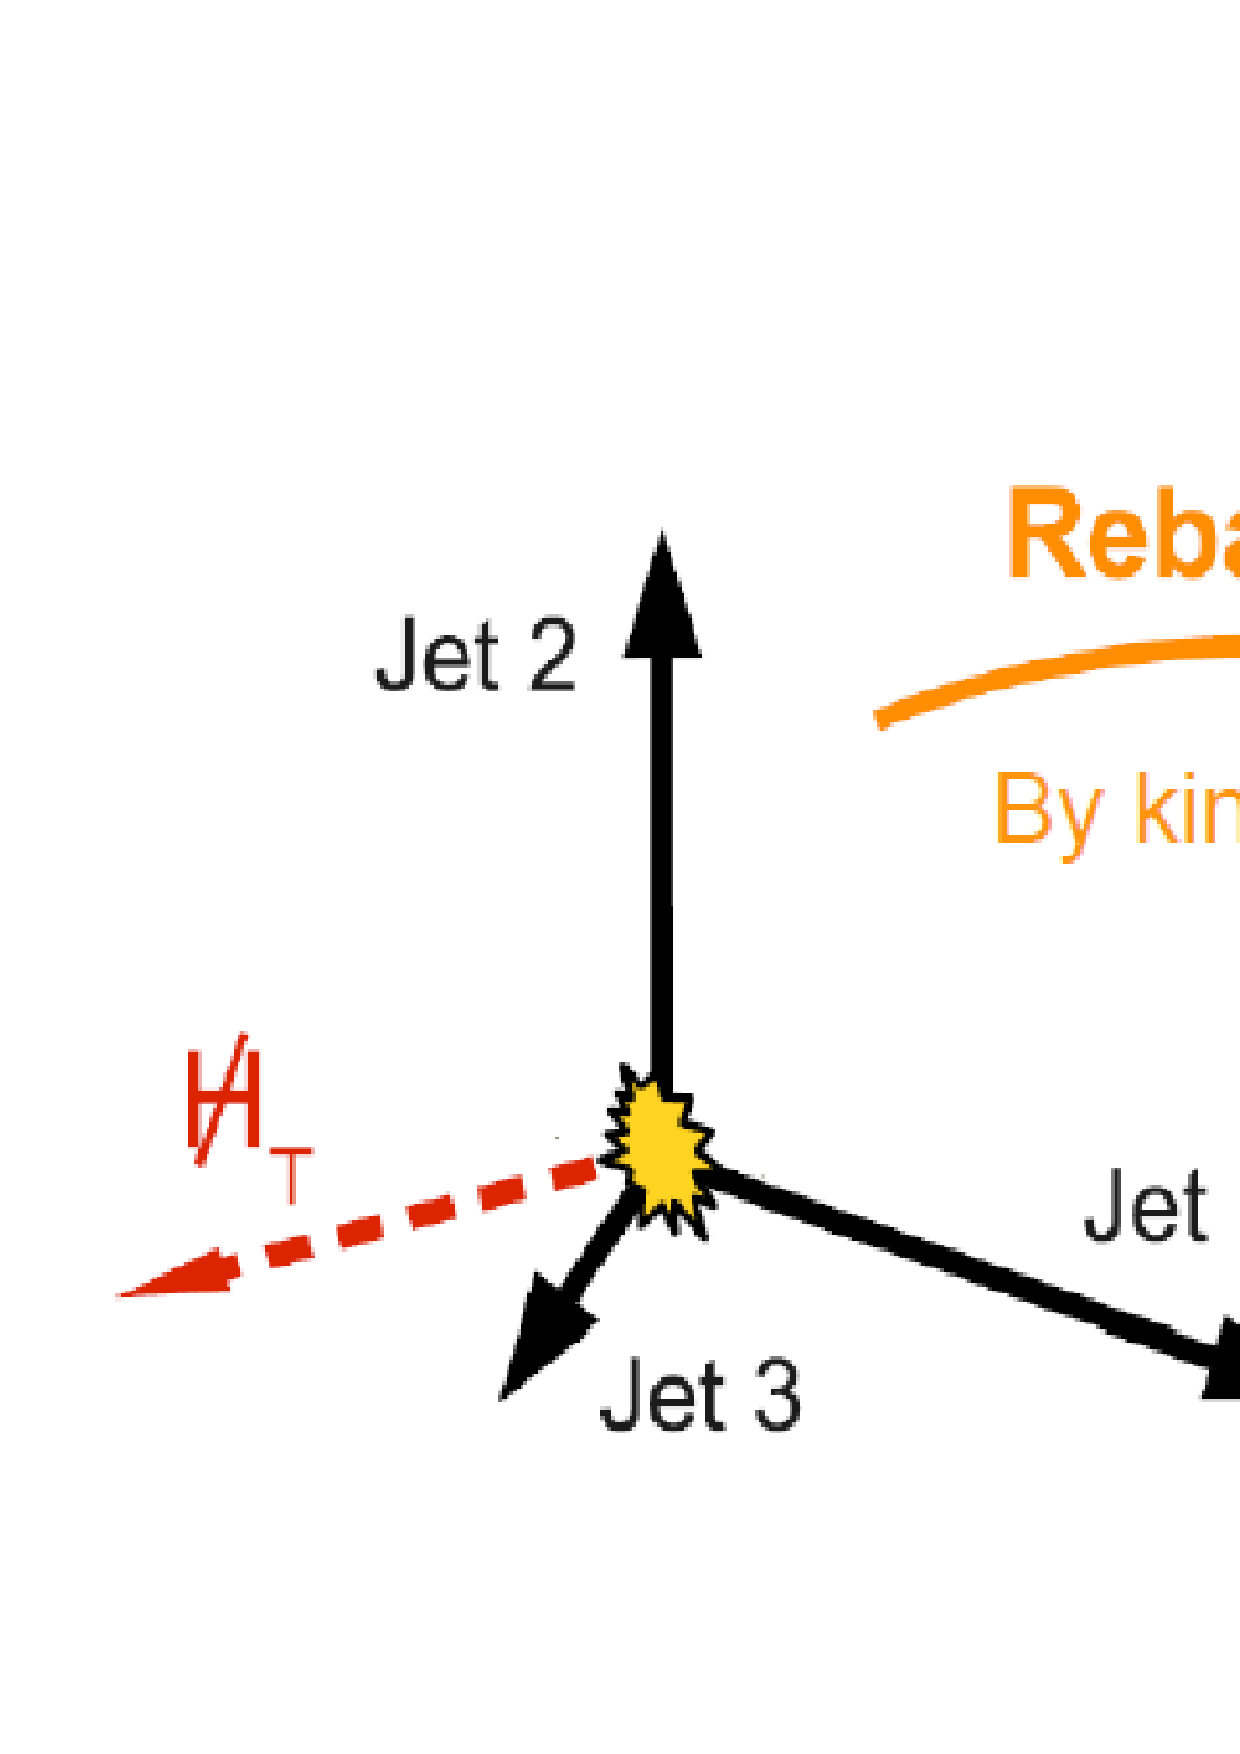
\includegraphics[width=0.99\textwidth]{figures/RPlusR.pdf}  
  \end{tabular}}
  \caption{Outline of the two steps performed in the R+S method for estimation of QCD background events~\cite{MSchrode}.}
  \label{fig:RPlusS_concept}
\end{figure}
\begin{description}
 \item \textbf{Reponse Templates:}
As indicated above, the R+S method crucially relies on a precise parametrization of the jet response to both perform the rebalancing and the jet smearing. The MC-truth response is derived for simulated events obtained with \pythia6 as well as \madgraph and the full detector simulation for $\pt^\mathrm{gen}$ and $|\eta^\mathrm{gen}|$ intervals summarized in Tab.~\ref{tab:RPlusS_binning}. Reconstructed jets at detector-level are calibrated according to the description in Sec.~\ref{subsec:jets_calib}. \\
As explained in Sec.~\ref{sec:jer_response}, the truth jet response is derived by performing an unambigous matching of reconstructed jet $i$ to generated jet $i$ using here $\Delta R < 0.1$. In addition, any further reconstructed or generated jet $j \ne i$ around this matched pair is vetoed in a cone of size $R < 0.7$ by requiring
\begin{equation}
 \pt^{\rm{GenJet}_j} / \pt^{\rm{GenJet}_i} < 0.05
\end{equation} 
and
\begin{equation}
 \pt^{\rm{Jet}_j} < 30\,\mathrm{GeV} \;\; \mathrm{and} \;\; \pt^{\rm{Jet}_j} / \pt^{\rm{Jet}_i} < 0.05
\end{equation} 
The obtained jet response distributions are averaged over all jets in an event not separating them according to their rank, \ie their position in a descending \pt order, or according to the jet flavour. Thus, the flavour composition reflects that of an average QCD multijet sample. 
\begin{table}[!t]
\centering
\caption{Overview of the $|\eta|$ and $\pt^{ave}$ interval boundaries used for the MC-truth response determination used as input for the R+S method.}
\label{tab:RPlusS_binning}
\makebox[\linewidth]{
\begin{tabular}{c}
\multicolumn{1}{c}{} \\
\toprule
 $|\eta^\mathrm{gen}|$ \\
 0, 0.3, 0.5, 0.8, 1.1, 1.4, 1.7, 2.0, 2.3, 2.8, 3.2, 4.1, 5.0 \\
\midrule
$\pt^\mathrm{gen} \; [\mathrm{GeV}]$ \\
0, 20, 30, 50, 80, 120, 170, 230, 300, 380, \\
470, 570, 680, 800, 1000, 1300, 1700, 2200, 2800, 3500 \\
\bottomrule
\end{tabular}}
\end{table} 
\\
The truth response templates to be used for applying the R+S method in simulated events, \eg for validation tests, are determined as described above. However, when using the truth response templates for the actual QCD background predictions in data, they have to be corrected for potential data to simulation jet resolution differences. As seen in Chap.~\ref{chap:Resolution}, the resolution in data is typically worse than in simulation. Thus, the determined truth response templates are adjusted accordingly. This correction is done for the Gaussian core and the non-Gaussian tails separately. First, the response function is splitted into the respective core and tail parts. This is done by fitting the response distribution with a Gaussian in the range of $\pm$ 1\,RMS around the mean which is then subtracted from the total response distribution in order to obtain the tail parts and vice versa. The correction factors for the core resolution are applied by convoluting the MC-truth response with a Gaussian of width $\sigma_{c}$ according to Eq.~\ref{eq:res_adjust}. The considered correction factors are listed in Tab.~\ref{tab:jer_RPlusS_core} in the appendix and correspond to the data-to-simulation ratios obtained from dijet data at $\sqrt{s} = 7$\tev, as illustrated in Fig.~\ref{fig:result_comparison} (right). Although the correction factors for the data-to-simulation ratio derived in the context of this thesis are more precise, these have not been available at that time when the analysis presented in this chapter has been performed. The residual tail contributions are scaled according to the correction factors $\rho_\mathrm{tail}$ listed in Tab.~\ref{tab:jer_RPlusS_tails} in the appendix derived from dijet asymmetry parts fulfilling $(\mathcal{A} > 2 \sigma_c)$~\cite{thesis:Schroeder}.   

 \item \textbf{Rebalance Procedure:}
Collision events are rebalanced in transverse momentum such that the missing transverse momentum is almost completely removed ($|\MHT^x| + |\MHT^y| < 0.02$) using a full kinematic fit. The jet momenta are allowed to vary in the fit according to the Gaussian core of the jet energy response. \\

 \item \textbf{Response Smearing:}
All jets of a rebalanced event are smeared with the full jet response templates including non-Gaussian tails obtained from simulated Monte Carlo samples. \\
The prediction of QCD contributions to the \HT and \MHT distributions are obtained using a bootstrap method \todo{ref}. Thus, each event is smeared $N = 100$ times. The mean of these N predictions is taken as final result while the statistical uncertainty is obtained as the standard deviation of this set of predictions \todo{formulas}.\\
In order to validate the smearing procedure, generated QCD events are smeared as described above and compared to fully simulated events at reconstruction level. The result of this generator jet smearing is shown in Fig.~\ref{fig:qcd_rs_genjets}. \\

\begin{figure}[hbtp]
  \centering
  \begin{tabular}{cc}
                \includegraphics[width=0.47\textwidth]{figures/HT_presel_madgraph_DR53X_chs_TuneZ2star_SmearedGenJets_withoutPUReweighting_v1.png} &
                \includegraphics[width=0.47\textwidth]{figures/NJets_baseline_withoutMHT_madgraph_DR53X_chs_TuneZ2star_SmearedGenJets_withoutPUReweighting_v1.png} 
  \end{tabular}
  \caption{Generated jets smeared with the truth response templates are compared to the expectation from full simulation. This comparison is shown for \HT (left) with a loose pre-selection of at least three jets and $N_{\text{jets}}$ (right) after the $\Delta \phi$ and the baseline \HT cut.}
  \label{fig:qcd_rs_genjets}
\end{figure}

The jet response templates do not incorporate a separation according to the heavy flavour composition of the sample since this composition depends on the jet rank and the templates are averaged over the rank of the jets. This leads to a potential non-closure of the method since light and heavy flavour jets are smeared with the same averaged response templates. In the end, this is covered by the uncertainty of the overall closure of the method. No additional uncertainty has to be assigned.
\end{description}

\subsection{Application to Realistic Collision Events}
\label{subsec:RPlusS_app} 
The presence of pile-up affects the rebalancing and needs to be taken particularly care of. Jets assigned to an event, especially soft jets, do not necessarily have to belong to the hard interaction, but might arise from pile-up events. Therefore, it is necessary to discard jets below a certain \pt threshold in the rebalancing step in order to not balance pile-up jets against the hard interaction. This \pt threshold can be chosen such that a good inclusive closure on Monte Carlo is observed. Nevertheless, by not taking all jets into account in the rebalancing, also soft jets belonging to the hard interaction are not considered. By doing this, additional imbalance in the event is introduced. It can be observed that this affects the kinematic fit such that especially jets with small \pt ($<$ 100 GeV) are on average rebalanced to too high momenta. This results then in the fact that more jets pass the threshold of 50 GeV than expected. As a consequence, the number of predicted QCD events in the higher jet multiplicity bins is too large. The resulting trend in the \NJets distribution for a \pt cut of 10\gev is illustrated in the left plot of Fig.~\ref{fig:qcd_rs_rebnjets}.\\

\begin{figure}[!t]
  \centering
  \begin{tabular}{cc}
                \includegraphics[width=0.47\textwidth]{figures/NJets_baseline_withoutMHT_madgraph_DR53X_chs_TuneZ2star_pt10_withoutPUReweighting_DoNotUseRebCorrection_v1.png} &
                \includegraphics[width=0.47\textwidth]{figures/NJets_baseline_withoutMHT_madgraph_DR53X_chs_TuneZ2star_pt10_withoutPUReweighting_UseRebCorrection_v1.png} 

  \end{tabular}
  \caption{Prediction of QCD background on a Monte Carlo sample compared to the expectation from full simulation showing the $N_{\text{jets}}$ distribution for a \pt cut of 10 GeV on jets considered in the rebalancing \textit{without} the application of a correction factor for the rebalancing (left) and \textit{with} a correction of the rebalancing procedure (right) as described in the text.}
  \label{fig:qcd_rs_rebnjets}
\end{figure}

In order to account for this unavoidable threshold effect, an empirical correction factor (f) is introduced. This is done by comparing the \pt-spectrum of the rebalanced jets to the \pt-spectrum of matched generated jets when rejecting jets below 10 GeV in the rebalancing procedure. The mean of this ratio is taken as correction factor and evaluated versus the momentum of the matched reconstructed jets. The correction factor is used such that in the rebalancing procedure each jet momentum is scaled by $1/\rm{f}$ before the kinematic fit is performed. This adjusted method then leads to correct predictions of the QCD event yields also in the high jet multiplicity bins as demonstrated in the right plot of Fig.~\ref{fig:qcd_rs_rebnjets}.\\
The correction factor is derived by using generator-truth information and hence can only be determined on Monte Carlo samples. This is performed on the flat PYTHIA QCD Monte Carlo sample and on the MADGRAPH Monte Carlo sample. The difference of the correction factors derived from these two samples is found to be of the order of $1-2\%$ cf. Fig.~\ref{fig:qcd_rs_rebfactor}, left. In addition, the correction factor was also determined for different bins of primary vertices and thus for different pile-up conditions. It is observed that the functional form of the correction factor is independent of the pile-up conditions cf. Fig.~\ref{fig:qcd_rs_rebfactor}, right. This justifies the assumption that the observed harder jet \pt-spectrum after the rebalancing without the correction factor is just due to the acceptance of the jet \pt cut on the jets considered for the rebalancing. Therefore, the correction factor derived from Monte Carlo is applied to data where the same \pt cut value of 10 GeV for jets considered in the rebalancing is chosen. Since a remaining non-closure of the method due to the rebalancing step is covered by the total non-closure uncertainty (discussed in Sec. ...), no additional uncertainty is assigned. 

\begin{figure}[!t]
  \centering
  \begin{tabular}{cc}
                \includegraphics[width=0.47\textwidth]{figures/RebalanceCorrectionFactors_DR53X_chsJets_TuneZ2star_withoutPUReweighting_pt10_vsRecoWithMadgraphComp.png} &
                \includegraphics[width=0.47\textwidth]{figures/RebalanceCorrectionFactors_DR53X_chsJets_TuneZ2star_withoutPUReweighting_pt10_vsRecoNVtxSplit.png}\\

  \end{tabular}
  \caption{Comparison of the rebalance correction factor determined on the PYTHIA and the MADGRAPH QCD Monte Carlo (left) and rebalance correction factor for different primary vertex bins (right).}
  \label{fig:qcd_rs_rebfactor}
\end{figure}

The quality of the R+S method to predict background contributions from QCD multijet events is tested on Monte Carlo samples by several closure tests in different kinematic regions. Therefore, the data-based prediction is applied to Monte Carlo events and compared to the results from full simulation. The different closure tests as function of \MHT for various jet multiplicity bins for a low \HT ($= 500 - 1000$~GeV) and a high \HT ($\ge 1000$~GeV) selection are shown in Fig.~\ref{fig:qcd_rs_closure}. These closure tests are used to determine the remaining bias of the R+S method. \\
The first choice for the determination of remaining biases is to calculate the difference between prediction and expectation for the signal region (defined by \MHT $>$~200 GeV and the application of the $\Delta \phi$ cut) and take the observed difference as systematic uncertainty or even correct the prediction for a statistically significant non-closure of the method. The calculated differences with their statistical errors for the signal region are summarized in Tab.~\ref{tab:qcd_rs_closure_unc} (left column). \\
There is one bin (for 3 -- 5 jets and \HT $= 500 - 1000$~GeV) where the signal region shows a statistically significant non-closure. In Fig.~\ref{fig:qcd_rs_closure_comp}, this particular distribution is shown for the MADGRAPH QCD sample (left) and the PYTHIA sample (right). In the region between \MHT $=$ 200 -- 350 GeV, the MADGRAPH sample shows an underprediction of $\approx 60\%$, while the PYTHIA sample tends to a statistically not significant overprediction. Therefore, it is hard to judge, if it is really a systematic effect or just a statistical fluctuation. In order to treat this conservatively, the result is not corrected for this effect, but the whole $60\%$ deviation in the madgraph sample is considered as systematic uncertainty. As QCD is not the dominant background contribution in this search bin, it will hardly affect the final result.\\
Since the number of events in the signal region is low for all bins except the one discussed above and thus the statistical uncertainties are large and do not lead to reasonable conclusions about the closure of the method, two sidebands of the signal region are studied. The prediction is compared to the full simulation either for control region 1 defined by \MHT $= 100 - 200$~GeV (second column in Tab.~\ref{tab:qcd_rs_closure_unc}) or for control region 2 defined by an inverted $\Delta \phi$ criterium (third column in Tab.~\ref{tab:qcd_rs_closure_unc}). 
\begin{itemize}
 \item If the differences in both control regions are statistically significant, the larger one is considered as systematic uncertainty. 
 \item If only one of the numbers is statistically significant, it has to be made sure that the assigned uncertainty by taking this number, e.g. coming from control region 1, is not too small, as a remaining bias might come from the application of the $\Delta \phi$ cut. Therefore, the chosen value is compared to the numbers in the corresponding cross check region bin (right column of Tab.~\ref{tab:qcd_rs_closure_unc}). If the values in the cross check region are smaller than the chosen uncertainty value from the control region, the number from the control region is considered as systematic error. Otherwise take largest number from cross check region.
 \item If none of the numbers is statistically significant, take the number with highest precision and proceed as above by comparing this value to the numbers in the cross check region. If the cross check region does not show larger values, take the number with highest precision, otherwise take largest number from cross check region.
\end{itemize}
The uncertainty which is then finally chosen by the procedure described above as the non-closure uncertainty of the method, is printed in bold letters in Tab.~\ref{tab:qcd_rs_closure_unc}.

\begin{figure}[h]
  \centering
  \begin{tabular}{cc}
                \includegraphics[width=0.45\textwidth]{figures/MHT_JetBin2_HTlow_madgraph_DR53X_chs_TuneZ2star_pt10_withoutPUReweighting_UseRebCorrection_v1.png} &
                \includegraphics[width=0.45\textwidth]{figures/MHT_JetBin2_HThigh_madgraph_DR53X_chs_TuneZ2star_pt10_withoutPUReweighting_UseRebCorrection_v1.png}\\
                \includegraphics[width=0.45\textwidth]{figures/MHT_JetBin3_HTlow_madgraph_DR53X_chs_TuneZ2star_pt10_withoutPUReweighting_UseRebCorrection_v1.png} &
                \includegraphics[width=0.45\textwidth]{figures/MHT_JetBin3_HThigh_madgraph_DR53X_chs_TuneZ2star_pt10_withoutPUReweighting_UseRebCorrection_v1.png}\\
                \includegraphics[width=0.45\textwidth]{figures/MHT_JetBin4_HTlow_madgraph_DR53X_chs_TuneZ2star_pt10_withoutPUReweighting_UseRebCorrection_v1.png} &
                \includegraphics[width=0.45\textwidth]{figures/MHT_JetBin4_HThigh_madgraph_DR53X_chs_TuneZ2star_pt10_withoutPUReweighting_UseRebCorrection_v1.png}\\

  \end{tabular}
  \caption{Prediction of QCD background on a Monte Carlo sample compared to the expectation from full simulation. The closure test is shown for various jet multiplicity bins and low (left) or high (right) \HT selections.}
  \label{fig:qcd_rs_closure}
\end{figure}

\begin{figure}[h]
  \centering
  \begin{tabular}{cc}
                \includegraphics[width=0.47\textwidth]{figures/MHT_JetBin2_HTlow_madgraph_DR53X_chs_TuneZ2star_pt10_withoutPUReweighting_UseRebCorrection_v1.png} &
                \includegraphics[width=0.47\textwidth]{figures/MHT_JetBin2_HTlow_pythia_DR53X_chs_TuneZ2star_pt10_withoutPUReweighting_UseRebCorrection_v1.png}\\
  \end{tabular}
  \caption{Prediction of QCD background on a Monte Carlo sample compared to the expectation from full simulation. The closure test is shown for 3 -- 5 jets and \HT $= 500 - 1000$~GeV on the madgraph QCD sample (left) and the pythia QCD sample (right).}
  \label{fig:qcd_rs_closure_comp}
\end{figure}

\begin{table}[h] 
  \centering
  \caption{Summary of non-closure uncertainties with their statistical error derived for the signal region (left) and two control regions with \MHT $= 100 - 200$~GeV (second column) and inverted $\Delta \phi$ criterium (third column). The fourth column is used as additional cross check region as described in the text. The numbers marked in bold letters are taken as the final non-closure uncertainties of the method.} 
  \label{tab:qcd_rs_closure_unc}
   \makebox[\linewidth]{
    \begin{tabular}{cc|cccc}
      \multicolumn{6}{c}{} \\
      \hline
      & & Signal region & Control region 1 & Control region 2 & Cross check region\\
      \hline
      $N_{\text{jets}}$ & \HT (GeV) & \MHT $>~200$ GeV &  \MHT $= 100 - 200$~GeV  &  \MHT $>~200$ GeV & \MHT $= 100 - 200$~GeV\\
      & & $\Delta \phi$ cut & $\Delta \phi$ cut & $\Delta \phi$ cut inverted & $\Delta \phi$ cut inverted\\
      \hline
      3 -- 5  & 500 -- 1000 & (\textbf{60.4} $\pm$~9.8)\% & (22.6 $\pm$~1.6)\% & (20.1 $\pm$~6.0)\% & (2.8 $\pm$~1.3)\%\\
      6 -- 7  & 500 -- 1000 & (43.1 $\pm$~46.5)\% & (\textbf{25.4} $\pm$~11.1)\% & (59.3 $\pm$~96.0)\% & (4.6 $\pm$~20.0)\%\\
      $\ge$ 8 & 500 -- 1000 & -- & (8.9 $\pm$~90.1)\% & (\textbf{86.0} $\pm$~38.2)\% & (12.2 $\pm$~66.4)\%\\
      \hline
      3 -- 5  & $\ge$ 1000 & (17.1 $\pm$~35.0)\% & (14.4 $\pm$~3.1)\% & (\textbf{14.5} $\pm$~8.9)\% & (5.1 $\pm$~1.7)\%\\
      6 -- 7  & $\ge$ 1000 & (5.5 $\pm$~108.0)\% & (\textbf{10.9} $\pm$~8.8)\% & (14.5 $\pm$~42.9)\% & (3.0 $\pm$~7.0)\%\\
      $\ge$ 8 & $\ge$ 1000 & (19.4 $\pm$~276.0)\% & (21.8 $\pm$~28.6)\% & (40.4 $\pm$~293.5)\% & (21.1 $\pm$~\textbf{42.6})\%\\
      \hline
    \end{tabular}}
\end{table}

Furthermore, the method can also be validated directly in data. The QCD background prediction is performed on a QCD enriched data control sample collected by a set of prescaled and unprescaled PFHT triggers. Thus, it has to be made sure that the events are collected such that the background prediction is not biased and the highest possible statistical precision is obtained. This is done as follows: For each event, the trigger with the lowest prescale is determined. The event then gets a weight according to this prescale factor. Since only one prescaled PFHT trigger exists, this assignment is unambigious. This leads to a smooth \HT spectrum going down to the lowest trigger threshold. The prescale weighted seed \HT distribution is shown in Fig.~\ref{fig:qcd_rs_seedht}.

\begin{figure}[h]
  \centering
  \begin{tabular}{c}
                \includegraphics[width=0.47\textwidth]{figures/HT_data.png}
  \end{tabular}
  \caption{Seed \HT spectrum of full 2012 dataset used as input for the R+S method after correcting for trigger prescales.}
  \label{fig:qcd_rs_seedht}
\end{figure}

The usage of prescaled triggers is important in order to collect also events with \HT lower than 500 GeV which enter the signal region through a fluctuation to large response values. Nevertheless the events collected by the prescaled trigger come along with high event weights and spoil artifically the prediction when they enter the signal region since they lead to a substantially higher standard deviation. This problem is solved by smearing the events not only $N = 100$ times, but $N = \rm{prescale~factor} \times 100$ times and weighting them accordingly with one.\\
\\
The performance of the R+S method can also be tested directly on data by comparing the prediction with selected data events in QCD enriched phase-space regions. This is done for \HT~$>~1000~\rm{GeV}$ and an inverted $\Delta \phi$ criterium in order to select a QCD enriched data sample as depicted in Fig.~\ref{fig:qcd_rs_dataclosure}. 
\begin{figure}[h]
  \centering
  \begin{tabular}{cc}
                \includegraphics[width=0.45\textwidth]{figures/HT_presel_HThigh_chsJets_535_Run2012ABCD_data_pt10_withUncertainties_UseRebCorrection_v3.png} &
                \includegraphics[width=0.45\textwidth]{figures/MHT_presel_HThigh_chsJets_535_Run2012ABCD_data_pt10_withUncertainties_UseRebCorrection_v3.png}\\
                \includegraphics[width=0.45\textwidth]{figures/Jet1Pt_presel_HThigh_chsJets_535_Run2012ABCD_data_pt10_withUncertainties_UseRebCorrection_v3.png} &
                \includegraphics[width=0.45\textwidth]{figures/Jet1Eta_presel_HThigh_chsJets_535_Run2012ABCD_data_pt10_withUncertainties_UseRebCorrection_v3.png}\\
                \multicolumn{2}{c}{\includegraphics[width=0.45\textwidth]{figures/NJets_presel_HThigh_chsJets_535_Run2012ABCD_data_pt10_withUncertainties_UseRebCorrection_v3.png}}
  \end{tabular}
  \caption{Prediction of QCD background on data compared to the expectation from data for a QCD enriched control region with \HT$>~1000~\rm{GeV}$, inverted $\Delta \phi$ cut and at least three jets.}
  \label{fig:qcd_rs_dataclosure}
\end{figure}
Nevertheless no perfect agreement is expected since contaminations from other backgrounds do still contribute. Especially the deviations in the \MHT distribution increase with increasing values of \MHT as QCD is not dominant here, so that a comparison is only reasonable for the low \MHT region. 


\subsection{Systematic Uncertainties}
\label{subsec:RA2_syst_unc}
Different uncertainties of the R+S method have been evaluated:
\begin{itemize}
\item \textbf{Core of response functions:} The uncertainties on the factors of the Gaussian core resolution in Tab.~\ref{tab:QCDJetRes:MLCoreScaleFactors} accounting for the differences in data and Monte Carlo are propagated to the prediction. This is done by shifting the scaling factors by $\pm 1\sigma$ up and down. The variations are between 10 to 30 $\%$ in the search bins where QCD leads to significant contributions.
\item \textbf{Tail of response functions:} The uncertainties on the scaling factors of the non-Gaussian tails are also propagated to the prediction. The typical size of this uncertainty in QCD dominated regions is between 20 to 35 $\%$ which results in the main systematic uncertainty of the method. 
\item \textbf{Non-closure:} The systematic uncertainty due to possible non-closure and remaining biases of the R+S method is evaluated as described in section \ref{sec:qcd_RS_closure}. This uncertainty also covers uncertainties on the rebalance correction factor and the jet-\pt cut value chosen for the jets considered in the rebalancing. It is evaluated for each jet multiplicity bin which is separated into a low and a high \HT $(>~1000~\rm{GeV})$ region.
\item \textbf{Pile-up:} In general, the R+S method is relatively safe against pile-up since very soft jets are neglected in the rebalancing procedure. Additionally, it is expected that pile-up is an issue especially for \textit{soft} jets which do not contribute significantly to the high \MHT search bins because they are mainly populated due to heavily mis-measured \textit{hard} jets. Therefore, a valid approach is to evaluate possible remaining pile-up effects in the low \MHT region for \MHT $> 100 \rm{~GeV}$. This approach also ensures that statistical limitations are reduced.\\
The general approach is to study the difference in the behaviour of the prediction in data and Monte Carlo for different pile-up conditions. Hence, the sample is divided into three different bins of primary vertices $(0-10, 11-20, > 20)$. The prediction for each vertex bin (for \HT $>~500$~GeV) is calculated and normalized to the number of seed events contributing to that particular bin. It is assumed that pile-up effects are negligible in the lowest primary vertex bin. Therefore the distributions in data and Monte Carlo are normalized to each other such that they have the same yield in the first primary vertex bin. Then, the absolute difference between data and Monte Carlo prediction is calculated for the second and the third vertex bin, multiplied each with the seed events in data for that bin and summed up. The input distributions for this calculation are illustrated in Fig.~\ref{fig:qcd_rs_pileup}. The ratio of this pile-up dependent fraction of the prediction calculated as described above and the total prediction is taken as pile-up uncertainty. It is evaluated for each jet multiplicity bin separately. 
\end{itemize}

\begin{figure}[hbtp]
  \centering
  \begin{tabular}{cc}
                \includegraphics[width=0.5\textwidth]{figures/PUUncertainty_NJet3_5.png} &
                \includegraphics[width=0.5\textwidth]{figures/PUUncertainty_NJet6_7.png} \\
                \multicolumn{2}{c}{\includegraphics[width=0.5\textwidth]{figures/PUUncertainty_NJet8.png}}
  \end{tabular}
  \caption{Prediction of QCD background in data and Monte Carlo as a function of primary vertices (NVtx) normalized to the number of contributing seed events used for the determination of the pile-up uncertainty as described in Sec.~\ref{sec:qcd_RS_uncertainty}.}
  \label{fig:qcd_rs_pileup}
\end{figure}

\subsection{QCD Background Prediction}
\label{subsec:RA2_qcd_pred}
The final prediction for QCD background contributions derived with the R+S method is summarized in tables~\ref{tab:qcd_rs_pred_njet3-5}, ~\ref{tab:qcd_rs_pred_njet6-7} and~\ref{tab:qcd_rs_pred_njet8} for jet multiplicity bins 3 --5, 6 --7 and $\ge 8$. The quoted total systematic uncertainty is obtained by adding the single contributions in quadrature. \\
Some search bins show very large uncertainties of 100 $\%$ or sometimes even larger for the core and tail scaling uncertainties. This occurs only in bins where QCD is almost negligible and is caused by the fact that the statistical variations are so large that they also dominate the evaluation of systematic effects. As a conservative estimate the largest observed variation is taken as systematic uncertainty for core and tail scaling. 

\begin{table}[htbp]
 \caption{Prediction of QCD background in 19.47 \fbinv for jet multiplicity 3 -- 5.}
 \label{tab:qcd_rs_pred_njet3-5}
  \begin{center}
    \begin{tabular} {c|c|c|c|c|c|c|c|c}
    \hline
    % \nJet $= 3 - 5$   \\
    %\hline
    HT (GeV) & MHT (GeV) & Pred. & Stat. & Core (\%) & Tail (\%) & Bias (\%) & PU (\%)& Tot. Sys. \\
    \hline
    500 - 800 & 200 - 300 & 307.4 & 18.48 & 13.03 & 35.95 & 60.4 & 2.9 & 219.93 \\ 
    & & & & -12.18 & -34.43 & -60.4 & -2.9 & 217.15 \\ 
    & 300 - 450 & 34.45 & 5.84 & 7.34 & 22.9 & 60.4 & 2.9 & 22.42 \\ 
    & & & & -10.48 & -31.58 & -60.4 & -2.9 & 23.78 \\ 
    & 450 - 600 & 1.32 & 1.15 & 24.24 & 37.88 & 60.4 & 2.9 & 0.99 \\ 
    & & & & -16.67 & -26.52 & -60.4 & -2.9 & 0.90 \\ 
    &  $>=$ 600 & 0.09 & 0.29 & 55.56 & 55.56 & 60.4 & 2.9 & 0.09 \\ 
    & & & & -55.56 & -55.56 & -60.4 & -2.9 & 0.09 \\ 
    \hline
    %800 - 1000 & 100 - 200 & 3.129e+04 & 184.2 & 19.96 & 11.69 & 22.6 & 2.9 & \\ 
    %& & & & -17.88 & -11.84 & -22.6 & -2.9 & \\ 
    800 - 1000 & 200 - 300 & 91.68 & 10.2 & 14.7 & 33.16 & 60.4 & 2.9 & 64.65 \\ 
    & & & & -13.83 & -33.53 & -60.4 & -2.9 & 64.65 \\ 
    & 300 - 450 & 9.94 & 3.22 & 5.23 & 29.78 & 60.4 & 2.9 & 6.72 \\ 
    & & & & -5.13 & -27.06 & -60.4 & -2.9 & 6.60 \\ 
    & 450 - 600 & 0.84 & 0.91 & 65.48 & 65.48 & 60.4 & 2.9 & 0.93 \\ 
    & & & & -65.48 & -65.48 & -60.4 & -2.9 & 0.84 \\ 
    &  $>=$ 600 & 0.12 & 0.35 & 75.00 & 8.33 & 60.4 & 2.9 & 0.12 \\ 
    & & & & -41.67 & -41.67 & -60.4 & -2.9 & 0.10 \\ 
    \hline
    %1000 - 1250 & 100 - 200 & 1.296e+04 & 115.1 & 18.57 & 10.39 & 14.5 & 2.9 & \\ 
    %& & & & -17.29 & -10.54 & -14.5 & -2.9 & \\ 
    1000 - 1250 & 200 - 300 & 59.00 & 7.20 & 19.03 & 34.71 & 14.5 & 2.9 & 24.93 \\ 
    & & & & -14.56 & -31.69 & -14.5 & -2.9 & 22.35 \\ 
    & 300 - 450 & 5.09 & 2.16 & 12.18 & 32.02 & 14.5 & 2.9 & 1.90 \\ 
    & & & & -8.84 & -16.9 & -14.5 & -2.9 & 1.23 \\ 
    & 450 - 600 & 0.51 & 0.67 & 35.29 & 23.53 & 14.5 & 2.9 & 0.23 \\ 
    & & & & -3.92 & -5.88 & -14.5 & -2.9 & 0.08 \\ 
    &  $>=$ 600 & 0.12 & 0.33 & 41.67 & 41.67 & 14.5 & 2.9 & 0.07 \\ 
    & & & & -41.67 & -41.67 & -14.5 & -2.9 & 0.07 \\ 
    \hline
    %1250 - 1500 & 100 - 200 & 4171 & 59.17 & 17.07 & 8.553 & 14.5 & 2.9 & \\ 
    %& & & & -16.23 & -9.374 & -14.5 & -2.9 & \\ 
    1250 - 1500 & 200 - 300 & 31.17 & 5.30 & 18.29 & 30.32 & 14.5 & 2.9 & 11.96 \\ 
    & & & & -19.12 & -29.68 & -14.5 & -2.9 & 11.93 \\ 
    & 300 - 450 & 2.27 & 1.27 & 16.3 & 38.33 & 14.5 & 2.9 & 1.00 \\ 
    & & & & -5.29 & -30.4 & -14.5 & -2.9 & 0.78 \\ 
    &  $>=$ 450 & 0.24 & 0.50 & 0.00 & 54.17 & 14.5 & 2.9 & 0.13 \\ 
    & & & & -8.33 & -8.33 & -14.5 & -2.9 & 0.05 \\ 
    \hline
    %$>=$ 1500 & 100 - 200 & 2350 & 48.78 & 14.87 & 7.565 & 14.5 & 2.9 & \\ 
    %& & & & -14.78 & -7.81 & -14.5 & -2.9 & \\ 
    $>=$ 1500 & 200 - 300 & 35.14 & 6.12 & 19.55 & 23.31 & 14.5 & 2.9 & 11.89 \\ 
    & & & & -19.98 & -29.43 & -14.5 & -2.9 & 13.54 \\ 
    &  $>=$ 300 & 2.43 & 1.37 & 39.92 & 39.92 & 14.5 & 2.9 & 1.42 \\ 
    & & & & -39.92 & -39.92 & -14.5 & -2.9 & 1.42 \\ 
    \hline
    \end{tabular}
  \end{center}
\end{table}

\begin{table}[htbp]
 \caption{Prediction of QCD background in 19.47 \fbinv for jet multiplicity 6 -- 7.}
 \label{tab:qcd_rs_pred_njet6-7}
  \begin{center}
    \begin{tabular} {c|c|c|c|c|c|c|c|c}
    \hline
    % \nJet $= 6 - 7$   \\
    %\hline
    HT (GeV) & MHT (GeV) & Pred. & Stat. & Core (\%) & Tail (\%) & Bias (\%) & PU (\%)& Tot. Sys. \\
    \hline
    500 - 800 & 200 - 300 & 18.19 & 3.85 & 8.91 & 37.38 & 25.4 & 8.0 & 8.50 \\ 
    & & & & -12.48 & -33.53 & -25.4 & -8.0 & 8.11 \\ 
    & 300 - 450 & 1.85 & 1.37 & 31.89 & 31.89 & 25.4 & 8.0 & 0.97 \\ 
    & & & & -31.89 & -31.89 & -25.4 & -8.0 & 0.97 \\ 
    &  $>=$ 450 & 0.01 & 0.10 & 400 & 400 & 25.4 & 8.0 & 0.06 \\ 
    & & & & -100 & -100 & -25.4 & -8.0 & 0.01 \\ 
    \hline
    %800 - 1000 & 100 - 200 & 3151 & 59.26 & 21.81 & 13.95 & 25.4 & 8.0 & \\ 
    %& & & & -18.72 & -13.73 & -25.4 & -8.0 & \\ 
    800 - 1000 & 200 - 300 & 13.13 & 3.40 & 15.00 & 33.74 & 25.4 & 8.0 & 5.98 \\ 
    & & & & -8.15 & -29.55 & -25.4 & -8.0 & 5.33 \\ 
    & 300 - 450 & 1.95 & 1.14 & 5.13 & 30.77 & 25.4 & 8.0 & 0.80 \\ 
    & & & & -20.00 & -28.21 & -25.4 & -8.0 & 0.85 \\ 
    &  $>=$ 450 & 0.15 & 0.39 & 46.67 & 46.67 & 25.4 & 8.0 & 0.11 \\ 
    & & & & -46.67 & -46.67 & -25.4 & -8.0 & 0.11 \\ 
    \hline
    %1000 - 1250 & 100 - 200 & 1853 & 40.37 & 19.92 & 12.29 & 10.9 & 8.0 & \\ 
    %& & & & -18.45 & -12.88 & -10.9 & -8.0 & \\ 
    1000 - 1250 & 200 - 300 & 11.92 & 3.84 & 5.87 & 33.47 & 10.9 & 8.0 & 4.36 \\ 
    & & & & -12.67 & -35.82 & -10.9 & -8.0 & 4.81 \\ 
    & 300 - 450 & 1.54 & 1.31 & 31.82 & 31.82 & 10.9 & 8.0 & 0.72 \\ 
    & & & & -31.82 & -31.82 & -10.9 & -8.0 & 0.72 \\ 
    &  $>=$ 450 & 0.11 & 0.32 & 100.00 & 100.00 & 10.9 & 8.0 & 0.16 \\ 
    & & & & -100.00 & -100.00 & -10.9 & -8.0 & 0.11 \\ 
    \hline
    %1250 - 1500 & 100 - 200 & 759.2 & 27.43 & 18.52 & 10.96 & 10.9 & 8.0 & \\ 
    %& & & & -18.19 & -11.52 & -10.9 & -8.0 & \\ 
    1250 - 1500 & 200 - 300 & 6.82 & 2.95 & 12.02 & 32.55 & 10.9 & 8.0 & 2.54 \\ 
    & & & & -11.88 & -32.40 & -10.9 & -8.0 & 2.53 \\ 
    & 300 - 450 & 0.92 & 1.03 & 54.35 & 54.35 & 10.9 & 8.0 & 0.72 \\ 
    & & & & -54.35 & -54.35 & -10.9 & -8.0 & 0.72 \\ 
    &  $>=$ 450 & 0.09 & 0.29 & 44.44 & 44.44 & 10.9 & 8.0 & 0.06 \\ 
    & & & & -44.44 & -44.44 & -10.9 & -8.0 & 0.06 \\ 
    \hline
    %$>=$ 1500 & 100 - 200 & 526.3 & 23.55 & 15.79 & 6.947 & 10.9 & 8.0 & \\ 
    %& & & & -16.86 & -10.42 & -10.9 & -8.0 & \\ 
    $>=$ 1500 & 200 - 300 & 8.0 & 2.84 & 20.9 & 31.54 & 10.9 & 8.0 & 3.13 \\ 
    & & & & -15.38 & -25.77 & -10.9 & -8.0 & 2.57 \\ 
    &  $>=$ 300 & 0.83 & 0.92 & 46.99 & 46.99 & 10.9 & 8.0 & 0.56 \\ 
    & & & & -46.99 & -46.99 & -10.9 & -8.0 & 0.56 \\ 
    \hline
    \end{tabular}
  \end{center}
\end{table}

\begin{table}[htbp]
 \caption{Prediction of QCD background in 19.47 \fbinv for jet multiplicity $\ge$ 8.}
 \label{tab:qcd_rs_pred_njet8}
  \begin{center}
    \begin{tabular} {c|c|c|c|c|c|c|c|c}
    \hline
    % \nJet $>= 8$   \\
    %\hline
    HT (GeV) & MHT (GeV) & Pred. & Stat. & Core (\%) & Tail (\%) & Bias (\%) & PU (\%)& Tot. Sys. \\
    \hline
    500 - 800 &  $>=$ 200 & 0.14 & 0.38 & 71.43 & 71.43 & 86.0 & 33.4 & 0.19 \\ 
    & & & & -71.43 & -71.43 & -86.0 & -33.4 & 0.14 \\ 
    \hline
    %800 - 1000 & 100 - 200 & 127.6 & 11.36 & 20.84 & 15.22 & 86.0 & 33.4 & \\ 
    %& & & & -16.67 & -14.35 & -86.0 & -33.4 & \\ 
    800 - 1000 &  $>=$ 200 & 0.54 & 0.69 & 33.33 & 33.33 & 86.0 & 33.4 & 0.56 \\ 
    & & & & -33.33 & -33.33 & -86.0 & -33.4 & 0.54 \\ 
    \hline
    %1000 - 1250 & 100 - 200 & 124 & 11.53 & 18.46 & 12.63 & 42.6 & 33.4 & \\ 
    %& & & & -20.06 & -14.16 & -42.6 & -33.4 & \\ 
    1000 - 1250 &  $>=$ 200 & 0.73 & 0.78 & 19.18 & 56.16 & 42.6 & 33.4 & 0.59 \\ 
    & & & & -1.37 & -27.4 & -42.6 & -33.4 & 0.44 \\ 
    \hline
    %1250 - 1500 & 100 - 200 & 71.07 & 8.204 & 19.39 & 13.37 & 42.6 & 33.4 & \\ 
    %& & & & -15.53 & -13.68 & -42.6 & -33.4 & \\ 
    1250 - 1500 &  $>=$ 200 & 0.54 & 0.75 & 55.56 & 55.56 & 42.6 & 33.4 & 0.52 \\ 
    & & & & -55.56 & -55.56 & -42.6 & -33.4 & 0.52 \\ 
    \hline
    %$>=$ 1500 & 100 - 200 & 64.96 & 7.861 & 16.04 & 8.544 & 42.6 & 33.4 & \\ 
    %& & & & -17.47 & -9.883 & -42.6 & -33.4 & \\ 
    $>=$ 1500 &  $>=$ 200 & 0.89 & 0.94 & 65.17 & 65.17 & 42.6 & 33.4 & 0.95 \\ 
    & & & & -65.17 & -65.17 & -42.6 & -33.4 & 0.89 \\ 
    \hline
    \end{tabular}
  \end{center}
\end{table}

\section{Results and Interpretation}
\label{sec:RA2_results}
\begin{table}[!t]
  \centering
  \caption{Predicted event yields for the different background components in the search regions defined by \HT, \MHT and \NJets. The uncertainties of the different background sources are added in quadrature to obtain the total uncertainties. Taken from~\cite{Chatrchyan:2014lfa}.
  }
  \label{tab:FinalEventYields}
  \makebox[\linewidth]{
    % \begin{tabular*}{\textwidth}{lll@{\extracolsep{\fill}}|r|r|r|r|r|r}
    \begin{tabular}{lll|r|r|r|r|r|r}
      \multicolumn{9}{c}{} \\
      \multicolumn{3}{c|}{Selection}
      & \multicolumn{1}{c|}{$Z \rightarrow \nu\bar{\nu}$} 
      & \multicolumn{1}{c|}{$\ttbar/W$}
      & \multicolumn{1}{c|}{$\ttbar/W$} 
      & \multicolumn{1}{c|}{QCD}
      & \multicolumn{1}{c|}{Total }
      & \multicolumn{1}{c}{Data}          \\

      \NJets{} & \HT{} [GeV] &\MHT{} [GeV]
      & \multicolumn{1}{c|}{} 
      & \multicolumn{1}{c|}{$\to \e,\mu+$X}
      & \multicolumn{1}{c|}{$\to \tau_{\mbox{\tiny h}}+$X}  
      & \multicolumn{1}{c|}{}
      & \multicolumn{1}{c|}{background}  
      & \multicolumn{1}{c}{}  \\ 
      % \hspace*{-2ex}
      \hline
      3-5     & 500-800    & 200-300  & 1821   $\pm$  387         & 2211   $\pm$  448        &1749   $\pm$  210        & 307  $\pm$  219         & 6088   $\pm$  665      &  6159  \\
      3-5     & 500-800    & 300-450  &  994   $\pm$  218         &  660   $\pm$  133        & 590   $\pm$   69        & 35   $\pm$   24         & 2278   $\pm$  266      &  2305  \\
      3-5     & 500-800    & 450-600  &  273   $\pm$   63         &   77   $\pm$   17        &  66.3 $\pm$   9.5       &  1.3 $^{+1.5}_{-1.3}$       & 418    $\pm$   66      &   454  \\
      3-5     & 500-800    & $>600$   &   42   $\pm$   10         &   9.5 $\pm$    4.0       &   5.7 $\pm$   1.3       &  0.1 $^{+0.3}_{-0.1}$       & 57.4   $\pm$   11.2    &    62  \\ \hline
      3-5     & 800-1000   & 200-300  &  216   $\pm$   46         &  278   $\pm$   62        & 192   $\pm$   33        & 92   $\pm$   66         & 777    $\pm$  107      &   808  \\
      3-5     & 800-1000   & 300-450  &  124   $\pm$   26         &  113   $\pm$   27        &  84   $\pm$   12        &  9.9 $\pm$    7.4       & 330    $\pm$   40      &   305  \\
      3-5     & 800-1000   & 450-600  &   47   $\pm$   11         &   36.1 $\pm$    9.9      &  24.1 $\pm$    3.6      &  0.8 $^{+1.3}_{-0.8}$       & 108    $\pm$   15      &   124  \\
      3-5     & 800-1000   & $>600$   &   35.3 $\pm$    8.8       &    9.0 $\pm$    3.7      &  10.3 $\pm$    2.0      &  0.1 $^{+0.4}_{-0.1}$       & 54.8   $\pm$   9.7     &    52  \\ \hline
      3-5     & 1000-1250  & 200-300  &   76   $\pm$   17         &  104   $\pm$   26        &  66.5 $\pm$    9.9      & 59   $\pm$   25         & 305    $\pm$   41      &   335  \\
      3-5     & 1000-1250  & 300-450  &   39.3 $\pm$    8.9       &   52   $\pm$   14        &  41   $\pm$   11        &  5.1 $\pm$    2.7       & 137    $\pm$   20      &   129  \\
      3-5     & 1000-1250  & 450-600  &   18.1 $\pm$    4.7       &    6.9 $\pm$    3.2      &   6.8 $\pm$    2.0      &  0.5 $^{+0.7}_{-0.5}$       & 32.3   $\pm$    6.1    &    34  \\
      3-5     & 1000-1250  & $>600$   &   17.8 $\pm$    4.8       &    2.4 $\pm$    1.8      &   2.5 $\pm$    0.8      &  0.1 $^{+0.3}_{-0.1}$       & 22.8   $\pm$    5.2    &    32  \\ \hline
      3-5     & 1250-1500  & 200-300  &   25.3 $\pm$    6.0       &   31.0 $\pm$    9.5      &  21.3 $\pm$    4.1      & 31   $\pm$   13         & 109    $\pm$   18      &    98  \\
      3-5     & 1250-1500  & 300-450  &   16.7 $\pm$    4.3       &   10.1 $\pm$    4.4      &  13.7 $\pm$    7.1      &  2.3 $\pm$    1.6       & 42.8   $\pm$    9.5    &    38  \\
      3-5     & 1250-1500  & $>450$   &   12.3 $\pm$    3.5       &    2.3 $\pm$    1.7      &   2.7 $\pm$    1.2      &  0.2 $^{+0.5}_{-0.2}$       & 17.6   $\pm$    4.1    &    23  \\ \hline
      3-5     & $>$1500    & 200-300  &   10.5 $\pm$    2.9       &   16.7 $\pm$    6.2      &  23.5 $\pm$    5.6      & 35   $\pm$   14         & 86     $\pm$   17      &    94  \\
      3-5     & $>$1500    & $>300$   &   10.9 $\pm$    3.1       &    9.7 $\pm$    4.3      &   6.6 $\pm$    1.4      &  2.4 $\pm$    2.0       & 29.7   $\pm$    5.8    &    39  \\ \hline \hline
      6-7     & 500-800    & 200-300  &   22.7 $\pm$    6.4       &  133   $\pm$   59        & 117   $\pm$   25        & 18.2 $\pm$    9.2       & 290    $\pm$   65      &   266  \\
      6-7     & 500-800    & 300-450  &    9.9 $\pm$    3.2       &   22   $\pm$   11        &  18.0 $\pm$    5.1      &  1.9 $\pm$    1.7       & 52     $\pm$   12      &    62  \\
      6-7     & 500-800    & $>450$   &    0.7 $\pm$    0.6       &    0.0 $^{+3.2}_{-0.0}$      &   0.1 $^{+0.5}_{-0.1}$      &  0.0 $^{+0.1}_{-0.0}$       & 0.8    $^{+3.3}_{-0.6}$    &     9  \\ \hline
      6-7     & 800-1000   & 200-300  &    9.1 $\pm$    3.0       &   56   $\pm$   25        &  46   $\pm$   11        & 13.1 $\pm$    6.6       & 124    $\pm$   29      &   111  \\
      6-7     & 800-1000   & 300-450  &    4.2 $\pm$    1.7       &   10.4 $\pm$    5.5      &  12.0 $\pm$    3.6      &  1.9 $\pm$    1.4       & 28.6   $\pm$    6.9    &    35  \\
      6-7     & 800-1000   & $>450$   &    1.8 $\pm$    1.0       &    2.9 $\pm$    2.5      &   1.2 $\pm$    0.8      &  0.1 $^{+0.4}_{-0.1}$       & 6.0    $\pm$    2.8    &     4  \\ \hline
      6-7     & 1000-1250  & 200-300  &    4.4 $\pm$    1.7       &   24   $\pm$   12        &  29.5 $\pm$    7.8      & 11.9 $\pm$    6.0       &  70    $\pm$   16      &    67  \\
      6-7     & 1000-1250  & 300-450  &    3.5 $\pm$    1.5       &    8.0 $\pm$    4.7      &   8.6 $\pm$    2.7      &  1.5 $\pm$    1.5       & 21.6   $\pm$    5.8    &    20  \\
      6-7     & 1000-1250  & $>450$   &    1.4 $\pm$    0.8       &    0.0 $^{+3.6}_{-0.0}$      &   0.6 $^{+0.8}_{-0.6}$      &  0.1 $^{+0.4}_{-0.1}$       & 2.2    $^{+3.8}_{-1.1}$    &     4  \\ \hline
      6-7     & 1250-1500  & 200-300  &    3.3 $\pm$    1.4       &   11.5 $\pm$    6.5      &   6.4 $\pm$    2.7      &  6.8 $\pm$    3.9       & 28.0   $\pm$    8.2    &    24  \\
      6-7     & 1250-1500  & 300-450  &    1.4 $\pm$    0.8       &    3.5 $\pm$    2.6      &   3.5 $\pm$    1.9      &  0.9 $^{+1.3}_{-0.9}$       & 9.4    $\pm$    3.6    &     5  \\
      6-7     & 1250-1500  & $>450$   &    0.4 $\pm$    0.4       &    0.0 $^{+2.5}_{-0.0}$      &   0.1 $^{+0.5}_{-0.1}$      &  0.1 $^{+0.3}_{-0.1}$       & 0.5    $^{+2.6}_{-0.4}$    &     2  \\ \hline
      6-7     & $>$1500    & 200-300  &    1.3 $\pm$    0.8       &   10.0 $\pm$    6.9      &   2.0 $\pm$    1.2      &  7.8 $\pm$    4.0       & 21.1   $\pm$    8.1    &    18  \\
      6-7     & $>$1500    & $>300$   &    1.1 $\pm$    0.7       &    3.2 $\pm$    2.8      &   2.8 $\pm$    1.9      &  0.8 $^{+1.1}_{-0.8}$       & 7.9    $\pm$    3.6    &     3  \\ \hline \hline 
      $\geq$8 & 500-800    & $>200$   &    0.0 $^{+0.8}_{-0.0}$       &    1.9 $\pm$    1.5      &   2.8 $\pm$    1.4      &  0.1 $^{+0.4}_{-0.1}$       & 4.8    $^{+2.3}_{-2.1}$    &     8  \\
      $\geq$8 & 800-1000   & $>200$   &    0.6 $\pm$    0.6       &    4.8 $\pm$    2.9      &   2.3 $\pm$    1.2      &  0.5 $^{+0.9}_{-0.5}$       & 8.3    $^{+3.4}_{-3.3}$    &     9  \\
      $\geq$8 & 1000-1250  & $>200$   &    0.6 $\pm$    0.5       &    1.4 $^{+1.5}_{-1.4}$      &   2.9 $\pm$    1.3      &  0.7 $^{+1.0}_{-0.7}$       & 5.6    $^{+2.3}_{-2.1}$    &     8  \\
      $\geq$8 & 1250-1500  & $>200$   &    0.0 $^{+0.9}_{-0.0}$       &    5.1 $\pm$    3.5      &   1.4 $\pm$    0.9      &  0.5 $^{+0.9}_{-0.5}$       & 7.1    $^{+3.8}_{-3.6}$    &     5  \\
      $\geq$8 & $>$1500    & $>200$   &    0.0 $^{+0.7}_{-0.0}$       &    0.0 $^{+4.2}_{-0.0}$      &   2.4 $\pm$    1.4      &  0.9 $^{+1.3}_{-0.9}$       & 3.3    $^{+4.7}_{-1.7}$    &     2  \\ \hline \hline


    \end{tabular}}
  % \end{lrbox}
  % \scalebox{0.95}{\usebox{\closureBox}}
  % }
  % \end{center}
\end{table}

The selected number of events in 19.5\fbinv of data together with the predicted event yields for the various SM background contributions estimated as discussed in Sec.~\ref{sec:RA2_Non-QCD} and Sec.~\ref{subsec:RA2_QCD} are listed in Tab.~\ref{tab:FinalEventYields} for all 36 exclusive search regions. The displayed uncertainties for the background predictions are the total uncertainties. These have been obtained by adding statistical and systematic uncertainties in quadrature. Furthermore, the obtained yields in data and the predicted background are visualized in Fig.~\ref{fig:ra2_summary}. The ratio in the bottom displayes the difference between observed data events and predicted background normalized to the background prediction. In general, the data are consistent with the SM expectation. The largest deviation occurs in the search region for $\NJets = 6-7$, $\HT = 500-800$\gev and $\MHT \ge 450$\gev. However, this is insignificant when including the probability to observe a statistical fluctuation as large or larger in any of the search regions. \\
\\
Since no significant excess over the SM prediction is observed, the results are interpreted in several simplified supersymmetric models of pair production of light-flavour squarks or gluinos. The LSP is denoted as $\tilde{\chi}_1^0$. Several different decay modes are studied in the parameter space of the LSP and the squark or gluino which are
\begin{description}
\item (a) $\tilde{q} \rightarrow q + \tilde{\chi}_1^0$
\end{description} 
in case of light-flavour squarks and
\begin{description}
\item (b) $\tilde{g} \rightarrow q\bar{q} + \tilde{\chi}_1^0$
\item (c) $\tilde{g} \rightarrow t\bar{t} + \tilde{\chi}_1^0$
\item (d) $\tilde{g} \rightarrow q\bar{q} + \tilde{\chi}_1^{\pm}/\tilde{\chi}_2^0 \;\; \mathrm{where} \;\; \tilde{\chi}_1^{\pm} \rightarrow W + \tilde{\chi}_1^0 \;\; \mathrm{and} \;\; \tilde{\chi}_2^0 \rightarrow Z + \tilde{\chi}_1^0$
\end{description}  
for decays of the gluino. The branching ratios are assumed to be 100\% for the different decay modes, except for case (d) where the decay via $\tilde{\chi}_1^{+}$, $\tilde{\chi}_1^{-}$ and $\tilde{\chi}_2^0$ is considered with equal probabilities. \\
Exclusion limits are derived with the modified $\mathrm{CL_s}$~\cite{0954-3899-28-10-313, Thomas1999435, bib:Higgs:CLS} approach \todo{CLs} and denote the 95\% confidence level (CL) upper limit on the production cross section of the signal. The profile likelihood ratio is used as test statistics which is derived from the combined likelihood of the acceptance, efficiencies and uncertainties for the signal as well as the background predictions for all search regions. The uncertainties considered for the signal acceptance and efficiency in the limit setting procedure are 
\begin{itemize} 
\item The uncertainty on the integrated luminosity amounts to 2.6\%~\cite{CMS-PAS-LUM-13-001}.
\item An uncertainty of 2\% is considered for a possible trigger inefficiency (cf. Sec.~\ref{subsec:RA2_samples_trigger}).
\item Due to the event cleaning criteria an uncertainty of 3\% is considered.
\item The propagation of the uncertainties on the jet energy calibration and resolution amount to uncertainties of $2-8$\% and $1-2\%$ in the signal acceptance, respectively. 
\item The systematic variation of PDFs~\cite{Botje:2011sn} leads to uncertainties of $1-8$\% in the signal acceptance. 
\item In order to match the maesured rate of initial-state radiation in data the simulation of the signal events is corrected accordingly~\cite{isrfsr}. For model parameter points with small differences between the LSP and the gluino or squark mass this results in an uncertainty of 22\% whereas it is usually less than a few percent for others.  
\end{itemize}
Finally, the resulting exclusion limits for the above described processes (a)-(d) are shown in Fig.~\ref{fig:ra2_limits}(a)-(d), respectively. The expected (\textit{dashed}) and observed (\textit{solid}) 95\% CL upper limits are shown accordingly in the gluino-LSP and squark-LSP mass plane for the signal production cross sections. The one-standard-deviation uncertainty for the theory prediction is obtained by varying the renormalization and factorization scale by a factor of two and incorporating CTEQ6.6~\cite{Nadolsky:2008zw} and MSTW2008~\cite{Martin:2009iq} as alternative PDF sets. By considering conservatively the observed limit minus the one sigma theory uncertainty, pair production of squarks of the first two generations is excluded below 780\gev for a LSP mass less than 200\gev. However, if only one light squark is accessible the limit decreases to 400\gev for LSP masses below 80\gev. Similarly, the pair production of gluinos could be excluded for the three different decay modes (b)-(d) in case of a LSP mass less than 100\gev for gluino masses up to 1.16\tev, 1.13\tev and 1.21\tev, respectively. 

\begin{figure}[!h]
  \centering
  \begin{tabular}{c}
    \includegraphics[width=0.99\textwidth]{figures/RA2_summary.pdf}
  \end{tabular}
  \caption{Summary of the observed number of events in each of the 36 search regions in comparison to the corresponding background prediction. The hatched region shows the total uncertainty of the background prediction. Taken from~\cite{Chatrchyan:2014lfa}.}
  \label{fig:ra2_summary}
\end{figure}

\begin{figure}[!h]
  \centering
  \begin{tabular}{cc}
                \includegraphics[width=0.49\textwidth]{figures/RA2_Limit1.pdf} &
                \includegraphics[width=0.49\textwidth]{figures/RA2_Limit2.pdf} \\
                \includegraphics[width=0.49\textwidth]{figures/RA2_Limit3.pdf} &
                \includegraphics[width=0.49\textwidth]{figures/RA2_Limit4.pdf} \\
  \end{tabular}
\caption{The observed and expected 95\% CL upper limits on the (a) squark-squark and (b-d) gluino-gluino production cross sections in either the m(squark)-m(LSP) or the m(gluino)-m(LSP) plane obtained with the simplified models. For the squark-squark production the upper set of curves corresponds to the scenario when the first two generations of squarks are degenerate and light, while the lower set corresponds to only one light accessible squark. Taken from~\cite{Chatrchyan:2014lfa}.} 
  \label{fig:ra2_limits}
\end{figure}

\subsection{Comparison to Other Measurements}
\label{subsec:RA2_comp}
The exclusion limits obtained with the analysis presented here exceed the exclusion limits derived from the 7\tev analysis (cf. Fig.~\ref{fig:SMS_7TeV}). Especially, the limit on the gluino mass is improved by around 200\gev for light LSPs. Furthermore, the extension of the analysis into the \NJets plane provided a good sensitivity towards the gluino-mediated production of third generation squarks and to decays involving $W$ and $Z$ bosons.

\begin{figure}[!h]
  \centering
\makebox[\linewidth]{
  \begin{minipage}[c]{1.\linewidth}
    \begin{center}
      \includegraphics[width=0.5\textwidth]{figures/T1_ICHEP2014_All.png}% \hspace {1.5 pt} 
      \includegraphics[width=0.5\textwidth]{figures/T2_ICHEP2014.png}\\ 
      \includegraphics[width=0.5\textwidth]{figures/T1tttt_ICHEP2014_All.png}
    \end{center}
  \end{minipage}}

  \caption{Comparison of various exclusion limits derived by different CMS analyses for the process $\tilde{g} \rightarrow q\bar{q} + \tilde{\chi}_1^0$ (\textit{top left}), $\tilde{q} \rightarrow q + \tilde{\chi}_1^0$ (\textit{top right}) and $\tilde{g} \rightarrow t\bar{t} + \tilde{\chi}_1^0$ (\textit{bottom}). Taken from~\cite{bib:CMS:PhysicsResultsSUS}}
  \label{fig:result_comp}
\end{figure}

%\begin{figure}[!tp]
%  \centering
%  \begin{tabular}{c}
%    \includegraphics[width=0.9\textwidth]{figures/T1_ICHEP2014_All.png}
%  \end{tabular}
%  \caption{Comparison of various exclusion limits derived by different CMS analyses for the SMS T1qqqq. Taken from ... (cms susy public results).}
%  \label{fig:T1_comp}
%\end{figure}

%\begin{figure}[!tp]
%  \centering
%  \begin{tabular}{c}
%    \includegraphics[width=0.9\textwidth]{figures/T2_ICHEP2014.png}
%  \end{tabular}
%  \caption{Comparison of various exclusion limits derived by different CMS analyses for the SMS T2qq. Taken from ... (cms susy public results).}
%  \label{fig:T1_comp}
%\end{figure}

%\begin{figure}[!tp]
%  \centering
%  \begin{tabular}{c}
%    \includegraphics[width=0.9\textwidth]{figures/T1tttt_ICHEP2014_All.png}
%  \end{tabular}
%  \caption{Comparison of various exclusion limits derived by different CMS analyses for the SMS T1tttt. Taken from ... (cms susy public results).}
%  \label{fig:T1_comp}
%\end{figure}

\section{Status of natural supersymmetry after LHC Run-I}
\label{sec:susy_status}


